\documentclass[10pt]{elegantbook}

\title{Reinforcement Learning Notes}
\subtitle{Learn from trying!}

\author{occupymars}
\date{June. 20, 2025}
\version{0.1}

\cover{iron_man.jpg}

% all the packages included
\usepackage{cprotect}
\usepackage{fontawesome}
\usepackage[linesnumbered, ruled]{algorithm2e}
\RestyleAlgo{algoruled}

% set some fonts
\setmonofont{Ubuntu Mono}
% \renewcommand{\arraystretch}{1.5}

% my own commands
% \newcommand{\mydefination}[1]{\textit{\textcolor[RGB]{0,174,247}{#1}}}
\newcommand{\mydefination}[1]{\textbf{\textit{\textcolor{structurecolor}{#1}}}}

\begin{document}

\maketitle

\frontmatter
\tableofcontents

\mainmatter

\chapter{Math of Reinforcement Learning}

\begin{introduction}
    \item Markov Decision Process
    \item Value Function
    \item Solving Value Function
    \item Action Value Function
    \item Bellman Optimality Equation
\end{introduction}
    
\section{Notation}
At some point I use $V^{\pi}$ to denote the value function under a certain policy $\pi$, but later I use $v_{\pi}$, they are the same.
It's a lagacy from my reading of the \textit{Dive into Deep Learning} book at first.

\section{Markov Decision Process}
\mydefination{State} and \mydefination{Action} can describe a robot state respect to the enviroment and actions to move around, 
$\mathcal S, \mathcal A$ are states and actions a robot can take, when taking an action, state after may not
be deterministic, it has a probability. We use a transition function $T: \mathcal S \times \mathcal A \times 
\mathcal S \rightarrow [0, 1]$ to denote this, $T(s, a, s') = p(s' \mid s,a)$ is the probability of reaching $s'$
given $s$ and $a$. For $\forall s \in \mathcal S$ and $\forall a \in \mathcal A$, $\sum_{s'\in S}T(s, a, s') = 1$. 

\mydefination{Reward} $r:\mathcal S \times \mathcal A \rightarrow \mathbb R$, $r(s,a)$ depends on current state and action. And the reward
may also be stochastic, given state and action, the reward has probability $p(r \mid s, a)$.

\mydefination{Policy} $\pi(a \mid s)$ tells agent which actions to take at every state, $\sum_a \pi(a \mid s) = 1$.

This can build a Markov Decision Process, $(\mathcal S, \mathcal A, \mathcal T, r)$ from the \mydefination{Trajectory} 
$\tau = (s_0, a_0, r_0, s_1, a_1, r_1, s_2, a_2, r_2, \ldots)$, which has probability of:
\[ p(\tau) = \pi(a_0\mid s_0) \cdot p(s_1 \mid s_0, a_0) \cdot \pi(a_1\mid s_1) \cdot p(s_2 \mid s_1, a_1) \cdots \] 

We then define \mydefination{Return} as the total reward $R(\tau) = \sum_t r_t$, 
the goal of reinforcement learning is to find a trajectory that has the largest return. The trajectory might be infinite, so in order for a 
meaningful formular of its return, we introduce a discount factor $\gamma < 1$, $R(\tau) = \sum_{t=0}^{\infty}\gamma^tr_t$. For large $\gamma$, 
the robot is encouraged to explore, for small one to take a short trajectory to goal.

Markov system only depend on current state and action, not the history one (but we can always augment the system).

\begin{remark}
    In this book, the reward to a state that is not forbidden and is not a boundary is set to 0. There are five actions: up, right, down, left, and stay, 
    with $a_1, \cdots, a_5$.
\end{remark}

\section{Value Function}
\mydefination{Value Function} is the value of a state, from that state, the expected sum reward (return). 

The formular of value function is:
\begin{equation}
    V^{\pi}(s_0) = \mathbb E_{a_t \sim \pi(s_t)}[R(\tau)] = \mathbb E_{a_t \sim \pi(s_t)}\left[ \sum_{t=0}^{\infty}\gamma^tr(s_t, a_t) \right]
\end{equation} 

If we divede the trajectory into two parts, $s_0$ and $\tau'$, we get the return:
\[ R(\tau) = r(s_0, a_0) + \gamma \sum_{t=1}^{\infty}\gamma^{t-1}r(s_t, a_t) = r(s_0, a_0) + \gamma R(\tau') \]

Put it back into the value function, using law of total expectation:
\[ \mathbb E[X] = \sum_a \mathbb E[X \mid A=a]p(a) = \mathbb E_a \left [\mathbb E[X \mid A=a] \right ] \]
we get:
\begin{equation}
    \begin{array}{lll}
    V^{\pi}(s_0) &=& \mathbb E_{a_t \sim \pi(s_t)}[r(s_0, a_0) + \gamma R(\tau')] \\
                 &=& \mathbb E_{a_0 \sim \pi(s_0)}[r(s_0, a_0)] + \gamma \mathbb E_{a_t \sim \pi(s_t)}[R(\tau')] \\
                 &=& \mathbb E_{a_0 \sim \pi(s_0)}[r(s_0, a_0)] + \gamma \mathbb E_{a_0 \sim \pi(s_0)}\left[\mathbb E_{s_1 \sim p(s_1 \mid a_0, s_0)}[\mathbb E_{a_t \sim \pi(s_t)}[R(\tau') \mid s_1, a_0]]\right] \\ 
                 &=& \mathbb E_{a_0 \sim \pi(s_0)}[r(s_0, a_0)] + \gamma \mathbb E_{a_0 \sim \pi(s_0)}\left[\mathbb E_{s_1 \sim p(s_1 \mid a_0, s_0)}[V^{\pi}(s_1)]\right] \\
                 &=& \mathbb E_{a \sim \pi(s)}\left[ r(s_0, a_0) + \gamma \mathbb E_{s_1 \sim p(s_1 \mid a_0, s_0)} [V^{\pi}(s_1)] \right]
    \end{array}
\end{equation}
before we put $s_1$ to the right as the condition, it is stochastic, inside the $E_{s_1 \sim p(s_1 \mid s_0, a_0)}$ scope it is deterministic, 
then we can get $V^{\pi}(s_1)$, as it needs the state to be deterministic.

The discrete formular is (get rid of the notation of time) so called \mydefination{Bellman Equation}:
\begin{equation} \label{eq:bellman_equation}
    V^{\pi}(s) = \sum_{a \in \mathcal A}\pi(a\mid s)\left[r(s,a) + \gamma \sum_{s'}p(s' \mid s, a)V^{\pi}(s')\right], \forall s \in S
\end{equation}

And if we write $r(s, a)$ as $\sum_r p(r \mid s, a) r$, then 
\[ p(r \mid s, a) = \sum_{s' \in \mathcal S}p(s', r \mid s, a) \]
We can also get
\[ p(s' \mid s, a) = \sum_{r \in \mathcal R} p(s', r \mid s, a) \]
combined we get
\begin{equation}
    V^{\pi}(s) = \sum_{a \in \mathcal A}\pi(a\mid s)\sum_{s' \in \mathcal S}\sum_{r \in \mathcal R}p(s', r \mid s, a)\left[r + \gamma V^{\pi}(s')\right]
\end{equation}

If the reward depend solely on the next state $s'$, then
\begin{equation}
    V^{\pi}(s) = \sum_{a \in \mathcal A}\pi(a\mid s)\sum_{s' \in \mathcal S}p(s' \mid s, a)\left[r(s') + \gamma V^{\pi}(s')\right]
\end{equation}

Let 
\begin{equation} \label{eq:bellman_equation_vector}
    \begin{array}{rll}
        r^{\pi}(s) &=& \sum_{a \in \mathcal A} \pi(a \mid s) \sum_r p(r \mid s, a) r \\
        p^{\pi}(s' \mid s) &=& \sum_{a \in \mathcal A} \pi(a \mid s) p(s' \mid s, a)
    \end{array}
\end{equation}
rewirte \ref{eq:bellman_equation} into the vector form:
\begin{equation}
    V^{\pi} = r^{\pi} + \gamma P^{\pi} V^{\pi}
\end{equation}
where $V^{\pi} = [V^{\pi}(s_1), \ldots, V^{\pi}(s_n)]^{\top} \in \mathbb R^n$, $r^{\pi} = [r^{\pi}(s_1), \ldots, r^{\pi}(s_n)]^{\top} \in \mathbb R^n$, and 
$P^{\pi} \in \mathbb R^{n \times n}$ with $P^{\pi}_{ij} = p^{\pi}(s_j \mid s_i)$.

\section{Solving Value Function} \label{sec:solving_value_function}
Next, we need to solve the value function, first way is closed-form solution:
\[ V^{\pi} = \left ( I - \gamma P^{\pi} \right )^{-1} r^{\pi} \]

Some properties: $I - \gamma P^{\pi}$ is invertible, $\left ( I - \gamma P^{\pi} \right )^{-1} \geq I$ which means every element of this inverse is nonnegative.
For every vector $r \geq 0$, it holds that $\left ( I - \gamma P^{\pi} \right )^{-1} r^{\pi} \geq r \geq 0$, so if $r_1 \geq r_2$, $\left ( I - \gamma P^{\pi} \right )^{-1} r_1^{\pi} \geq
\left ( I - \gamma P^{\pi} \right )^{-1} r_2^{\pi}$

However, this method need to calculate the inverse of the matrix, that need some numerical algorithms. We can 
use a iterative solution:
\[ V_{k+1} = r^{\pi} + \gamma P^{\pi}V_k \]
as $k \rightarrow \infty$, $V_k \rightarrow V^{\pi} = \left ( I - \gamma P^{\pi} \right )^{-1} r^{\pi}$.

\begin{proof}
    Define the error as $\delta_k = V_k - V^{\pi}$, substitute $V_{k+1} = \delta_{k+1} + V^{\pi}$ and $V_k = \delta_k + V^{\pi}$ into the equation:
    \[ \delta_{k+1} + V^{\pi} = r^{\pi} + \gamma P^{\pi}(\delta_k + V^{\pi}) \]
    Rearrange it:
    \[ 
    \begin{array}{lll}
        \delta_{k+1} &=& r^{\pi} + \gamma P^{\pi}V^{\pi} + \gamma P^{\pi}\delta_k - V^{\pi} \\
        &=& \gamma P^{\pi}V^{\pi} + r^{\pi} + \gamma P^{\pi}\delta_k - V^{\pi} \\
        &=& \gamma P^{\pi}\delta_k
    \end{array}
    \]
    As a result, $\delta_{k+1} = \gamma P^{\pi} \delta_k = (\gamma P^{\pi})^2 \delta_{k-1} = \cdots = (\gamma P^{\pi})^{k+1} \delta_0$.
    Since every entry of $P^{\pi}$ is nonnegative and no greater than 1, and $\gamma < 1$, we have $\|(\gamma P^{\pi})^{k+1}\| \rightarrow 0$ as $k \rightarrow \infty$,
    and the error $\|\delta_k\| \rightarrow 0$ as $k \rightarrow \infty$.
\end{proof}

\section{Action Value Function}
Similarly to value funtion, \mydefination{Action Value Function} is the value of an action at state s, 
from that state, take that action, the expected sum reward (return). We use $V^{\pi}(s)$ to denote value function, 
and $Q^{\pi}(s,a)$ to denote action value, their connection is:
\begin{equation}
    V^{\pi}(s) = \sum_{a \in \mathcal A}\pi(a\mid s) Q^{\pi}(s,a)
\end{equation} 

The action value function is given as:
\begin{equation}
    \begin{array}{lll}
    Q^{\pi}(s_0, a_0) &=& r(s_0, a_0) + \mathbb E_{a_t \sim \pi(s_t)}\left[ \sum_{t=1}^{\infty}\gamma^tr(s_t, a_t) \right] \\
                      &=& r(s_0, a_0) + \gamma \mathbb E_{a_t \sim \pi(s_t)}\left[ \sum_{t=1}^{\infty}\gamma^{t-1} r(s_t, a_t) \right] \\
                      &=& r(s_0, a_0) + \gamma \mathbb E_{a_t \sim \pi(s_t)}[R(\tau ')] \\
                      &=& r(s_0, a_0) + \gamma \mathbb E_{s_1 \sim p(s_1 \mid s_0, a_0)} \left [ \mathbb E_{a_t \sim \pi(s_t)}[R(\tau ') \mid s_1] \right ] \\
                      &=& r(s_0, a_0) + \gamma \mathbb E_{s_1 \sim p(s_1 \mid s_0, a_0)} [V^{\pi}(s_1)] \\
                      &=& r(s_0, a_0) + \gamma \mathbb E_{s_1 \sim p(s_1 \mid s_0, a_0)} \left [\sum_{a_1 \in \mathcal A}\pi(a_1 \mid s_1) Q^{\pi}(s_1, a_1) \right ]
    \end{array}
\end{equation} 

Then the bellman equation of action value is:
\begin{equation} \label{eq:bellman_equation_action}
    \begin{array}{lll}
    Q^{\pi}(s, a) &=& r(s, a) + \gamma \sum_{s'}p(s' \mid s, a)V^{\pi}(s') \\
                  &=& r(s, a) + \gamma \sum_{s'}p(s' \mid s, a)\sum_{a' \in \mathcal A}\pi(a' \mid s')Q^{\pi}(s', a')
    \end{array}
\end{equation} 
Note that we can always write $r(s, a)$ as $\sum_r p(r \mid s, a) r$ if it is stochastic, and it follows the same notation
in the book \textit{Math of Reinforcement Learning}.

Rewrite \ref{eq:bellman_equation_action} into vector form:
\begin{equation}
    Q^{\pi} = \tilde r + \gamma P \Pi Q^{\pi}
\end{equation}
where $\tilde r_{(s,a)} = \sum_r p(r \mid s, a)r$, 
$P_{(s, a), s'} = p(s' \mid s, a)$, $\Pi_{s', (s', a')} = \pi(a' \mid s')$.

\section{Bellman Optimality Equation}
\begin{definition}[Optimal Policy]
    If $V^{\pi_1}(s) \geq V^{\pi_2}(s), \forall s \in \mathcal S$, than $\pi_1$ is better than $\pi_2$, if $\pi_1$ is better than all other policies, 
it is called \mydefination{Optimal Policy} $\pi^*$.
\end{definition}

\mydefination{Bellman Optimality Equation} (BOE) is given by:
\begin{equation} \label{eq:bellman_optimality_equation}
    \begin{array}{lll}
    V(s) &=& \max_{\pi(s) \in \Pi(s)} \sum_{a \in \mathcal A}\pi(a\mid s) \big ( \sum_r p(r \mid s, a) r + \gamma \sum_{s'}p(s' \mid s, a)V(s') \big ) \\
         &=& \max_{\pi(s) \in \Pi(s)} \sum_{a \in \mathcal A}\pi(a\mid s) Q(s, a)
    \end{array}
\end{equation}

There are two unknowns in the equation, $V(s)$ and $\pi(a \mid s)$, we can first consider the right hand side, to compute the $\pi(a \mid s)$.
\begin{example}
    Consider $\sum_{1}^{3} c_i q_i$, where $c_1 + c_2 + c_3 = 1$ and they are all greater than 0, without loss of generality, we can assume $q_3 \geq q_1, q_2$, 
    then the maximum is achieved when $c_3 = 1, c_1 = 0, c_2 = 0$. This is beacuse:
    \[ q_3 = (c_1 + c_2 + c_3)q_3 = c_1 q_3 + c_2 q_3 + c_3 q_3 \geq c_1 q_1 + c_2 q_2 + c_3 q_3 \]
\end{example}

Inspired by the example, since $\sum_a \pi(a \mid s) = 1$, we have:
\[ \sum_{a \in \mathcal A}\pi(a \mid s) Q(s, a) \leq \sum_{a \in \mathcal A}\pi(a \mid s)\max_{a \in \mathcal A} Q(s, a) = \max_{a \in \mathcal A} Q(s, a) \]
where the equality is achieved when
\[
\pi(a \mid s) = \left \{ 
\begin{array}{l}
    1, \quad a = a^*, \\
    0, \quad a \neq a^*.
\end{array} \right .
\]
here $a^* = \arg\max_{a \in \mathcal A} Q(s, a)$.

Then the matrix form of BOE is:
\[ V = \max_{\pi \in \Pi} (r^{\pi} + \gamma P^{\pi}V) = f(V) \]
the $r^{\pi}$ and $P^{\pi}$ are the same before in normal Bellman equation \ref{eq:bellman_equation_vector}.

In order to solve this nonlinear equation, we first need to introduce \mydefination{Contraction Mapping} theorem or Fixed Point theorem:
\begin{definition}[Contraction Mapping]
    Consider function $f(x)$, where $x \in \mathbb R^d$ and $f:\mathbb R^d \rightarrow \mathbb R^d$. A point $x^*$ is called a fixed point if 
    $f(x^*) = x^*$, and the function is a contraction mapping if there exists $\gamma \in (0, 1)$ such that:
    \[ \| f(x_1) - f(x_2) \| \leq \gamma \| x_1 - x_2 \|, \forall x_1, x_2 \in \mathbb R^d \] 
\end{definition}

The relation between a fixed point and the contraction property is characterized by:
\begin{theorem}[Banach's Fixed Point Theorem]
    For any equation that has the form $x = f(x)$ where $x$ and $f(x)$ are real vectors, if $f$ is a contraction mapping, than:
    \begin{enumerate}
        \item Existence: There exists a fixed point $x^*$ such that $f(x^*) = x^*$.
        \item Uniqueness: There exists a unique fixed point $x^*$ such that $f(x^*) = x^*$.
        \item Algorithm: For any initial point $x_0$, the sequence $x_{k+1} = f(x_k)$ converges to the fixed point $x^*$.
        Moreover, the convergence rate is exponentially fast.
    \end{enumerate}
\end{theorem}

The proof of the theorem can be found in the book, it is based on Cauthy sequence. Then we need to show the right hand side of the BOE is a contraction mapping:
\begin{theorem}[Contraction Property of right-hand side of BOE]
    For any $V_1, V_2 \in \mathbb R^{|\mathcal S|}$, it holds that:
    \[ \| f(V_1) - f(V_2) \|_{\infty} \leq \gamma \| V_1 - V_2 \|_{\infty} \]
    where $\gamma \in (0, 1)$ is the discount factor, $\| \cdot \|_{\infty}$ is the maximum norm, which is the
maximum absolute value of the elements of a vector.
\end{theorem}

\begin{proof}
    \begin{align*}
        f(V_1) = \max_{\pi} (r^{\pi} + \gamma P^{\pi}V_1) = r^{\pi^*_1} + \gamma P^{\pi^*_1}V_1 \geq r^{\pi^*_2} + \gamma P^{\pi^*_2}V_1 \\
        f(V_2) = \max_{\pi} (r^{\pi} + \gamma P^{\pi}V_2) = r^{\pi^*_2} + \gamma P^{\pi^*_2}V_2 \geq r^{\pi^*_1} + \gamma P^{\pi^*_1}V_2
    \end{align*}
    where $\geq$ is elementwise comparison, as a result:
    \[ 
    \begin{array}{lll}
        f(V_1) - f(V_2) &=& (r^{\pi^*_1} - r^{\pi^*_2}) + \gamma P^{\pi^*_1}V_1 - \gamma P^{\pi^*_2}V_2 \\
                        &\leq& (r^{\pi^*_1} - r^{\pi^*_1}) + \gamma P^{\pi^*_1}V_1 - \gamma P^{\pi^*_1}V_2 \\
                        &=& \gamma P^{\pi^*_1}(V_1 - V_2) \\
    \end{array}    
    \]
    similarly we can get $f(V_2) - f(V_1) \leq \gamma P^{\pi^*_2}(V_2 - V_1)$, so we have:
    \[ \gamma P^{\pi^*_2}(V_1 - V_2) \leq f(V_1) - f(V_2) \leq \gamma P^{\pi^*_1}(V_1 - V_2) \]
    define
    \[ z = \max \big \{ | \gamma P^{\pi^*_1}(V_1 - V_2) |, | \gamma P^{\pi^*_2}(V_1 - V_2) | \big \} \in \mathbb R^{|\mathcal S|} \]
    all the operations are elementwise, $z \geq 0$, then we have:
    \[ -z \leq \gamma P^{\pi^*_2}(V_1 - V_2) \leq f(V_1) - f(V_2) \leq \gamma P^{\pi^*_1}(V_1 - V_2) \leq z \]
    which imlies:
    \[ |f(V_1) - f(V_2)| \leq z \]
    it then follows that:
    \begin{equation} \label{eq:BOE_proof}
        \| f(V_1) - f(V_2) \|_{\infty} \leq \| z \|_{\infty}
    \end{equation}
    suppose $z_i, p_i^T, q_i^T$ are $i$th entry of $z, P^{\pi^*_1}, P^{\pi^*_2}$, then:
    \[ z_i = \max \big \{ |\gamma p_i^T(V_1 - V_2)|, |\gamma q_i^T(V_1 - V_2)| \big \} \]
    since $p_i$ sums up to 1 and nonnegative, we have:
    \[ |p_i^T (V_1 - V_2) | \leq p_i^T |V_1 - V_2| \leq \| V_1 - V_2 \|_{\infty} \]
    similarly we have $|q_i^T (V_1 - V_2) | \leq \| V_1 - V_2 \|_{\infty}$, therefore $z_i \leq \gamma \| V_1 - V_2 \|_{\infty}$, and hence
    \[ \| z \|_{\infty} = \max_i |z_i| \leq \gamma \| V_1 - V_2 \|_{\infty} \]
    Substitute it back to \ref{eq:BOE_proof}, we have:
    \[ \| f(V_1) - f(V_2) \|_{\infty} \leq \gamma \| V_1 - V_2 \|_{\infty} \]
\end{proof}

Then we can use this to solve an optimal policy from the BOE. Since $V^* = \max_{\pi \in \Pi} (r^{\pi} + \gamma P^{\pi}V^*)$, so it is clearly a 
fixed point.

\begin{theorem}[Existence, Uniqueness and Algorithm of Optimal Policy]
    The optimal policy $V^*$ exists and is unique, and the sequence $V_{k+1} = f(V_k)$ converges to the optimal policy $V^*$ exponentially fast
    given any initial guess $V_0$ with the iteration algorithm:
    \[ V_{k+1} = f(V_k) = \max_{\pi \in \Pi} (r^{\pi} + \gamma P^{\pi}V_k) \]
\end{theorem}

The proof follows the proof of the contraction mapping theorem, and the iteration algorithm is called \mydefination{Value Iteration}.
Once we have the optimal value function $V^*$, we can get the optimal policy $\pi^*$ by:
\begin{equation}
    \pi^* = \arg\max_{\pi \in \Pi} (r^{\pi} + \gamma P^{\pi}V^*)
\end{equation}
substitute this into the BOE yields $V^* = r^{\pi^*} + \gamma P^{\pi^*}V^*$, which is the optimal value function.

\begin{theorem}[Optimality of Value Function and Policy]
    The solution $V^*$ and the policy $\pi^*$ are optimal, i.e., for any other policy $\pi \in \Pi$, it holds that:
    \[ V^* = V^{\pi^*} \geq V^{\pi} \] 
\end{theorem}

\begin{proof}
    \[ V^* - V^{\pi} = r^{\pi^*} + \gamma P^{\pi^*}V^* - r^{\pi} - \gamma P^{\pi}V^{\pi} \geq 
    r^{\pi} + \gamma P^{\pi}V^* - r^{\pi} - \gamma P^{\pi}V^{\pi} = \gamma P^{\pi} (V^* - V^{\pi}) \]
    iteratively we have $V^* - V^{\pi} \geq \lim_{n \rightarrow \infty} (\gamma P^{\pi})^n (V^* - V^{\pi})$.
\end{proof}

\begin{theorem}[Greedy optimal policy]
    For any $s \in \mathcal S$, the deterministic greedy policy:
    \begin{equation} \label{eq:greedy_policy}
        \pi(a \mid s) = \left \{ 
        \begin{array}{l}
            1, \quad a = a^*, \\
            0, \quad a \neq a^*.
        \end{array} \right .
    \end{equation}
    is an optimal policy, where $a^* = \arg\max_{a \in \mathcal A} Q^{*}(s, a)$, where
    \[ Q^{*}(s, a) = \sum_{r \in \mathcal R}p(r \mid s, a)r + \gamma \sum_{s'}p(s' \mid s, a)V^{*}(s') \]
    remember that even though $V^*$ is unique, the optimal policy may not be unique, and there always exists a greedy optimal policy.
\end{theorem}

We can talk about the impact of the reward values:
\begin{theorem}[Optimal policy invaraince]
    If every reward $r \in \mathcal R$ is changed by an affine transformation to $\alpha r + \beta$, where $\alpha, \beta \in \mathbb R$ and $\alpha > 0$, then
the corresponding optimal state value $V'$ is also an affine transformation of $V^*$:
\[ V' = \alpha V^* + \frac{\beta}{1 - \gamma} \mathbf{1} \]
Consequently, the optimal policy derived from $V'$ is invariant to the affine transformation of the reward values.
\end{theorem}

And with the discount factor $\gamma$, the optimal policy will not take any meaningless detour.

\section{Value Iteration and Policy Iteration}
The algorithm of \mydefination{Value Iteration} is:
\[ V_{k+1} = \max_{\pi \in \Pi} (r^{\pi} + \gamma P^{\pi}V_k) \]
and there are two steps in one iteration, first one is called \mydefination{Policy Update}:
\[ \pi_{k+1} = \arg\max_{\pi \in \Pi} (r^{\pi} + \gamma P^{\pi}V_k) \]
the second one is called \mydefination{Value Update}:
\[ V_{k+1} = r^{\pi_{k+1}} + \gamma P^{\pi_{k+1}}V_k \]

With the elementwise form, the policy update is (if there are same actions that takes the maximum, we can choose any of them):
\[ \pi_{k+1}(s) = \arg\max_{\pi(s) \in \Pi(s)} \sum_{a \in \mathcal A}\pi(a\mid s) \big ( \sum_r p(r \mid s, a) r + \gamma \sum_{s'}p(s' \mid s, a)V_k(s') \big ) \]
Then the value update is:
\[ V_{k+1}(s) = \sum_{a \in \mathcal A}\pi_{k+1}(a\mid s) \big ( \sum_r p(r \mid s, a) r + \gamma \sum_{s'}p(s' \mid s, a)V_k(s') \big ) \]
We can use the greedy deterministic policy, which is then:
\[ V_{k+1}(s) = \max_a Q_k(s, a) \]

We should know that $V_k$ is not a state value though it converges to the optimal state value, it is not ensured to satisfy the Bellman equation. So the 
$Q_k$ is also not a action value, they are all intermediate values.

The algorithm of \mydefination{Policy Iteration} has also two steps, first one is called \mydefination{Policy Evaluation}:
\[ V^{\pi_k} = r^{\pi_k} + \gamma P^{\pi_k}V^{\pi_k} \]
second one is called \mydefination{Policy Improvement}:
\[ \pi_{k+1} = \arg\max_{\pi \in \Pi} (r^{\pi_k} + \gamma P^{\pi_k}V^{\pi_k}) \]

Here comes the first question, how to solve the policy evaluation? We can use the iterative method introduced in \ref{sec:solving_value_function}, and this 
results an iteration algorithm inside an iteration algorithm. We will not do infinite iteration here, so the $V^{\pi_k}$ will not be the exact solution, would 
this cause problem? No, see the truncated policy iteration algorithm.

And the second question, why $\pi_{k+1}$ is better than $\pi_{k}$?
\begin{lemma}[Policy Improvement] \label{lemma:policy_improvement}
    If $\pi_{k+1} = \arg\max_{\pi \in \Pi} (r^{\pi_k} + \gamma P^{\pi_k}V^{\pi_k})$, then $V^{\pi_{k+1}}(s) \geq V^{\pi_{k}}(s), \forall s \in \mathcal S$.
\end{lemma}
\begin{proof}
    We know that:
    \[ r^{\pi_{k+1}} + \gamma P^{\pi_{k+1}}V^{\pi_{k+1}} \geq r^{\pi_k} + \gamma P^{\pi_k}V^{\pi_k} \]
    Then
    \[
    \begin{array}{lll}
        V^{\pi_k} - V^{\pi_{k+1}} &=& r^{\pi_k} + \gamma P^{\pi_k}V^{\pi_k} - (r^{\pi_{k+1}} + \gamma P^{\pi_{k+1}}V^{\pi_{k+1}}) \\
        & \leq & r^{\pi_{k+1}} + \gamma P^{\pi_{k+1}}V^{\pi_k} - (r^{\pi_{k+1}} + \gamma P^{\pi_{k+1}}V^{\pi_{k+1}}) \\
        & \leq & \gamma P^{\pi_{k+1}}(V^{\pi_k} - V^{\pi_{k+1}})
    \end{array}
    \]
    again iteratively we have:
    \[ V^{\pi_k} - V^{\pi_{k+1}} \leq \lim_{n \rightarrow \infty} (\gamma P^{\pi_{k+1}})^n (V^{\pi_k} - V^{\pi_{k+1}}) = 0 \]
\end{proof}

\begin{theorem}[Convergence of policy iteration]
    The state value sequence $\{ V^{\pi_k} \}_{k=0}^{\infty}$ converges to the optimal state value $V^*$, and the policy sequence $\{ \pi_k \}_{k=0}^{\infty}$ 
    converges to the optimal policy $\pi^*$ in policy iteration algorithm.
\end{theorem}
\begin{proof}
    We introduce another sequence $\{ V_{k} \}_{k=0}^{\infty}$ generated by:
    \[ V_{k+1} = f(V_k) = \max_{\pi} (r^{\pi} + \gamma P^{\pi} V_k) \]
    which is exactly the value iteration algorithm, and we know that $V_k \rightarrow V^*$ as $k \rightarrow \infty$.
    For $k = 0$, we can always find a $V_0$ such that $V_0 \leq V^{\pi_0}$, then we use induction: for $k \geq 0$, if $V_k \leq V^{\pi_k}$, then for $k+1$:
    \begin{align*}
        V^{\pi_{k+1}} - V_{k+1} 
        &= \left(r^{\pi_{k+1}} + \gamma P^{\pi_{k+1}} V^{\pi_{k+1}}\right) - \max_{\pi} \left(r^{\pi} + \gamma P^{\pi} V_k\right) \\
        &\geq \left(r^{\pi_{k+1}} + \gamma P^{\pi_{k+1}} V_k\right) - \max_{\pi} \left(r^{\pi} + \gamma P^{\pi} V_k\right) \\
        &\quad \text{(because } V^{\pi_{k+1}} \geq V_k \text{ by Lemma \ref{lemma:policy_improvement} and } P^{\pi_{k+1}} \geq 0 \text{)} \\
        &= \left(r^{\pi_k'} + \gamma P^{\pi_k'} V_k\right) - \left(r^{\pi_k'} + \gamma P^{\pi_k'} V_k\right) \\
        &\quad \text{(suppose } \pi_k' = \arg\max_{\pi} \left(r^{\pi} + \gamma P^{\pi} V_k\right)) \\
        &\geq \left(r^{\pi_k'} + \gamma P^{\pi_k'} V_k\right) - \left(r^{\pi_k'} + \gamma P^{\pi_k'} V_k\right) \\
        &\quad \text{(because } \pi_{k+1} = \arg\max_{\pi} \left(r^{\pi} + \gamma P^{\pi} V_k\right)) \\
        &= \gamma P^{\pi_k'} \left(V_{k+1} - V_k\right) \geq 0 \\
    \end{align*}
    Since $V_k$ converges to $V^*$, $V^{\pi_k}$ is also converges to $V^*$.
\end{proof}

Then the elementwise form of the policy iteration algorithm is, policy evaluation:
\[ V^{\pi_k}_{(j+1)}(s) = \sum_{a \in \mathcal A}\pi_{k+1}(a\mid s) \big ( \sum_r p(r \mid s, a) r + \gamma \sum_{s'}p(s' \mid s, a)V^{\pi_k}_{(j)}(s') \big ) \]
and policy improvement:
\[ \pi_{k+1}(s) = \arg\max_{\pi(s) \in \Pi(s)} \sum_{a \in \mathcal A}\pi(a\mid s) \big ( \sum_r p(r \mid s, a) r + \gamma \sum_{s'}p(s' \mid s, a)V^{\pi_k}(s') \big ) \]

Next we introduce \mydefination{Truncated Policy Iteration} algorithm, which is a combination of value iteration and policy iteration. We will
see that the value iteration and policy iteration algorithms are two special cases of the truncated policy iteration algorithm.

If we start from $V_0^{\pi_1} = V_0$, we get:
\[
\begin{array}{rll}
    && V^{(0)}_{\pi_1} = V_0 \\
    \text{value iteration} & \leftarrow V_1 \leftarrow & V_{(1)}^{\pi_1} = r^{\pi_1} + \gamma P^{\pi_1} V_{(0)}^{\pi_1} \\
    && V_{(2)}^{\pi_1} = r^{\pi_1} + \gamma P^{\pi_1} V_{(1)}^{\pi_1} \\
    && \vdots \\
    \text{truncated policy iteration} & \leftarrow \bar{V}_1 \leftarrow & V_{(j)}^{\pi_1} = r^{\pi_1} + \gamma P^{\pi_1} V_{(j-1)}^{\pi_1} \\
    && \vdots \\
    \text{policy iteration} & \leftarrow V^{\pi_1} \leftarrow & V_{(\infty)}^{\pi_1} = r^{\pi_1} + \gamma P^{\pi_1} V_{(\infty)}^{\pi_1}
\end{array}
\]

\begin{figure}[htbp]
    \centering
    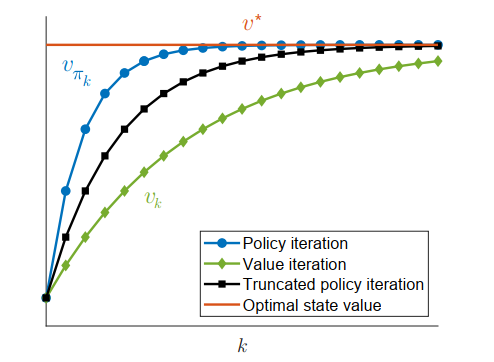
\includegraphics[width=0.60\textwidth]{image/3_iteration.png}
    \caption{3 iteration methods}
    \label{fig:3_iteration}
\end{figure}

\begin{proposition}[Value Improvement]
    In the policy evaluation step if the initial guess is selected as $V^{\pi_k}_{(0)} = V^{\pi_{k-1}}$, then it holds that:
    \[ V^{\pi_k}_{(j+1)} \geq V^{\pi_k}_{(j)} \]
\end{proposition}

\begin{proof}
    \[ V^{\pi_k}_{(j+1)} - V^{\pi_k}_{(j)} = \gamma P^{\pi_k} (V^{\pi_k}_{(j)} - V^{\pi_k}_{(j-1)}) = \cdots = \gamma^j P^{\pi_k} (V^{\pi_k}_{(1)} - V^{\pi_k}_{(0)}) \]
    we have
    \[ V^{\pi_k}_{(1)} = r^{\pi_k} + \gamma P^{\pi_k} V^{\pi_{k-1}} \geq r^{\pi_{k-1}} + \gamma P^{\pi_{k-1}} V^{\pi_{k-1}} = V^{\pi_{k-1}} = V^{\pi_{k}}_{(0)} \]
    where the inequality is due to $\pi_k = \arg\max_{\pi} (r^{\pi} + \gamma P^{\pi} V^{\pi_{k-1}})$, substitute $V^{\pi_{k}}_{(1)} \geq V^{\pi_{k}}_{(0)}$ into 
    the first equation, we have $V^{\pi_k}_{(j+1)} \geq V^{\pi_k}_{(j)}$.
\end{proof}

But we have to note that this is based on the assumption that the initial guess is $V^{\pi_k}_{(0)} = V^{\pi_{k-1}}$, 
and $V^{\pi_{k-1}}$ is not always available, like in the truncated policy iteration algorithm, we do not do the iteration until convergence, 
but only do a few steps, so the initial value is approximation. And in Deep Reinforcement Learning, we do not have the exact value function, 
even if we have it may not be tranferable or meaningful.



\section{Monte Carlo Method}
If we sample from a independent and identically distributed (i.i.d.) distribution, we can use the Monte Carlo method to do mean estimate, as value function 
ans action value function are all mean estimates.

In the policy iteration, the action value lies in the core of these two steps, we first use Bellman equation to compute the value function, then use it 
to compute action value, and then update the policy. If we do not have a model, than the definition of action value is:
\[ Q^{\pi_k}(s, a) = \mathbb E[G_t | S_t = s, A_t = a] = \mathbb E[R_{t+1} + \gamma R_{t+2} + \gamma^2 R_{t+3} + \dots | S_t = s, A_t = a] \]
we use $R$ to denote the stochastic reward, and $G_t$ is the return at time $t$.

If we run the policy for $n$ episodes than we get:
\begin{equation}
    Q^{\pi_k}(s, a) = \mathbb E[G_t | S_t = s, A_t = a] \approx \frac{1}{n} \sum_{i=1}^{n} G^{\pi_k}_{(i)}(s, a)
\end{equation}
instead of calculation of value function, we directly get action value from samples, this is the simplest Monte Carlo method (we call it MC Basic).

In the example of the book, we can see that if the length of the episodes are too short, it will get zero action value, because it can not get to 
the target. This is caused by the \mydefination{Sparse Reward}.

We next show how to efficiently use the samples. Every time a state-action pair appears in an episodes, it is called a \textit{visit}.
Given an episodes:
\[ s_1 \xrightarrow{a_2} s_2 \xrightarrow{a_4} s_1 \xrightarrow{a_2} s_2 \xrightarrow{a_3} s_5 \xrightarrow{a_1} \dots \]

\begin{enumerate}
    \item Initial visit, only the first pair is evaluated, like in the MC Basic, which is not efficient.
    \item First-visit, only use the samples to estimate the action value of the first visit.
    \item Every visit, use the samples to estimate the action value of every visit, which is more efficient, but may cause bias (because they are subsequence
    , there are corrleation).
\end{enumerate}

Then we consider how to efficiently update the policy.
\begin{enumerate}
    \item In the policy evaluation step, to collect all the episodes starting from the same state-action pair and then approximate the action value using the
average return of these episodes, which is in MC Basic. The drawback of this strategy is that the agent must wait until all the episodes have
been collected before the estimate can be updated.
    \item Use the return of a single episode to approximate the corresponding action value. In this way, we can
immediately obtain a rough estimate when we receive an episode. Then, the policy can be improved in an episode-by-episode fashion. In fact, this strategy
falls into the scope of \mydefination{Generalized Policy Iteration} introduced in the last chapter,we can still update the policy even if the value estimate is not sufficiently accurate.
\end{enumerate}

So the new algorithm is called \mydefination{MC Exploring Starts}, based on the exploring starts condition, which means that the agent can start from any state 
and take any action (MC Basic assume this too).

\begin{algorithm}[H]
\caption{MC Exploring Starts (efficient variant of MC Basic)}
\KwIn{Initial policy $\pi_0(a|s)$, $Q(s,a)$, $\text{Returns}(s,a)=0$, $\text{Num}(s,a)=0, \forall (s,a)$}

\ForEach{episode}{
    \textbf{Episode generation:} Select $(s_0,a_0)$ (exploring-starts), then generate $s_0,a_0,r_1,\dots,s_{T-1},a_{T-1},r_T$ following $\pi$ \\
    $g \gets 0$ \\
    \For{$t=T-1, T-2, \dots, 0$}{
        $g \gets \gamma g + r_{t+1}$ \\
        $\text{Returns}(s_t,a_t) \gets \text{Returns}(s_t,a_t) + g$ \\
        $\text{Num}(s_t,a_t) \gets \text{Num}(s_t,a_t) + 1$ \\
        $Q(s_t,a_t) \gets \frac{\text{Returns}(s_t,a_t)}{\text{Num}(s_t,a_t)}$ \\
        $\pi(a|s_t) \gets \begin{cases}
        1 & \text{if } a = \arg\max_a Q(s_t,a), \\
        0 & \text{otherwise}
        \end{cases}$
    }
}
\end{algorithm}

\vspace{\baselineskip}

We can see that the algorithm starts from the last state of the episode, and then update the action value and policy in a \textbf{reverse order}.

However, the exploring starts condition is not always satisfied, for example in the real world involving physical interactions, we need to remove this 
condition. A policy is \textbf{soft} if it has a positive probability of taking any action at any state, with a soft policy, a single
episode that is sufficiently long can visit every state-action pair many times. Thus we do not need the exploring starts condition.

One type of soft policy is \mydefination{$\epsilon$-greedy Policy}:
\begin{equation}
    \pi(a \mid s) = \left \{ 
    \begin{array}{l}
        1 - \frac{\epsilon}{|\mathcal A(s)|}(|\mathcal A(s)| - 1), \text{for the greedy action}, \\
        \frac{\epsilon}{|\mathcal A(s)|}, \text{for the other actions}.
    \end{array} \right .
\end{equation}
Where $\pi \in \Pi_{\epsilon}$ is the set of all $\epsilon$-greedy policies, and $|\mathcal A(s)|$ is the number of actions available at state $s$.
The probability of taking the greedy action is always greater than that of taking any other action. 

With this we can change the policy improvement step:
\begin{equation} \label{eq:e_greedy_policy}
    \pi(a \mid s) = \left \{ 
    \begin{array}{l}
        1 - \frac{\epsilon}{|\mathcal A(s)|}(|\mathcal A(s)| - 1), \quad a = a^*, \\
        \frac{\epsilon}{|\mathcal A(s)|}, \quad a \neq a^*.
    \end{array} \right .
\end{equation}

So the algorithm is:

\begin{algorithm}[H]
\caption{MC $\epsilon$-greedy (a variant of MC Exploring Starts)}
\KwIn{Initial policy $\pi_0(a|s)$, $Q(s,a)$, $\text{Returns}(s,a)=0$, $\text{Num}(s,a)=0, \forall (s,a). \epsilon \in (0, 1]$}

\ForEach{episode}{
    \textbf{Episode generation:} Select $(s_0,a_0)$, then generate $s_0,a_0,r_1,\dots,s_{T-1},a_{T-1},r_T$ following $\pi$ \\
    $g \gets 0$ \\
    \For{$t=T-1, T-2, \dots, 0$}{
        $g \gets \gamma g + r_{t+1}$ \\
        $\text{Returns}(s_t,a_t) \gets \text{Returns}(s_t,a_t) + g$ \\
        $\text{Num}(s_t,a_t) \gets \text{Num}(s_t,a_t) + 1$ \\
        $Q(s_t,a_t) \gets \frac{\text{Returns}(s_t,a_t)}{\text{Num}(s_t,a_t)}$ \\
        $\pi(a|s_t) \gets \begin{cases}
        1 - \frac{\epsilon}{|\mathcal A(s)|}(|\mathcal A(s)| - 1) & a = a^*, \\
        \frac{\epsilon}{|\mathcal A(s)|} & a \neq a^*.
        \end{cases}$
    }
}
\end{algorithm}

\vspace{\baselineskip}

The policy is optimal in $\Pi_{\epsilon}$, not in $\Pi$, so it is not guaranteed to be optimal, but it is still a good policy (if $\epsilon$ is sufficiently small).


\section{Stochastic Approximation}
For now, we only learned non-incremental algorithms, which may take a logn time to compute, not good for online learning.
Suppose $w_{k} = \frac{1}{k-1} \sum_{i=1}^{k-1} x_i, k = 2, 3, \ldots$, then:
\[ w_{k+1} = \frac{1}{k} \sum_{i=1}^{k} x_i = \frac{k-1}{k} w_k + \frac{1}{k} x_k \]
this update the mean estimate incrementally. We use 
\begin{equation}
    w_{k+1} = w_{k} - \alpha_k (w_{k} - x_k)
\end{equation}
$\alpha_k$ may not be given, though 
above we give it as $\frac{1}{k}$.

Given a noisy observation of $g(w)$:
\[ \tilde{g}(w, \eta) = g(w) + \eta \]
where $\eta$ is a noise, we can use the stochastic approximation method \mydefination{Robbins-Monro} algorithm to update the estimate of $w$:
\begin{equation}
    w_{k+1} = w_k - \alpha_k \tilde{g}(w_k, \eta_k), \alpha_k > 0
\end{equation}

Why this algorithm converge?
\begin{theorem}[Robbins-Monro theorem] \label{theorem:RM}
    If
    \begin{enumerate}
        \item $0 \leq c_1 \leq \nabla_{w}g(w) \leq c_2 < \infty$, $\forall w$; So $g$ is monotonic and bounded;
        \item $\sum_{k=1}^{\infty} \alpha_k = \infty$ and $\sum_{k=1}^{\infty} \alpha_k^2 < \infty$; It should converge to zero, but not too fast, one 
        common choice is $\alpha_k = \frac{1}{k}$;
        \item $\mathbb E[\eta_k \mid \mathcal H_k] = 0$ and $\mathbb E[\eta_k^2 \mid \mathcal H_k] < \infty$;
    \end{enumerate}
    where $\mathcal H_k = \{ w_k, w_{k-1}, \ldots, \}$, then $w_k$ converges to the root of $g(w)$ almost surely, i.e., 
    $\lim_{k \rightarrow \infty} w_k = w^*$, where $g(w^*) = 0$.
\end{theorem}

Then let $g(w) = w - \mathbb E[X], \tilde g(w, \eta) = w - x + \eta, \eta = \mathbb E[X] - x$, 
we can use the Robbins-Monro algorithm to prove that with careful choice of $\alpha_k$, the estimate $w_k$ converges to the mean $\mathbb E[X]$ almost surely.

\begin{theorem}[Dvoretzky's Theorem]
    Consider a stochastic sequence:
    \[ \Delta_{k+1} = (1 - \alpha_k) \Delta_k + \beta_k \eta_k \]
    where $\alpha_k, \beta_k \geq 0$, then  $\Delta_k$ converges to 0 almost surely, if:
    \begin{enumerate}
        \item $\sum_{k=1}^{\infty} \alpha_k = \infty$, $\sum_{k=1}^{\infty} \alpha_k^2 < \infty$, and $\sum_{k=1}^{\infty} \beta_k^2 < \infty$ uniformly almost surely;
        \item $\mathbb E[\eta_k \mid \mathcal H_k] = 0$ and $\mathbb E[\eta_k^2 \mid \mathcal H_k] < \infty$ almost surely.
    \end{enumerate}
    where $\mathcal H_k = \{ \Delta_k, \Delta_{k-1}, \ldots, \eta_{k-1}, \ldots, \alpha_{k-1}, \ldots, \beta_{k-1}, \ldots, \}$.
    
    In RM, $\alpha_k, \beta_k$ are deterministic, but in Dvoretzky's theorem, they can be stochastic, and is useful in cases they are function of $\Delta_k$.
\end{theorem}

\begin{proof}
    Please refer to the book, page 110.
\end{proof}

And we can also use this theorem to prove the convergence of the mean estimation, Robbins-Monro algorithm as well, and please refer to the book too.

\begin{theorem}[Exentsion of Dvoretzky's Theorem] \label{theorem:extension_dvoretzky}
    Consider a finite set $\mathcal S$ of real numbers, a stochastic process:
    \[ \Delta_{k+1}(s) = (1 - \alpha_k(s)) \Delta_k(s) + \beta_k(s) \eta_k(s) \]
    $\Delta_k(s)$ converges to 0 almost surely, if:
    \begin{enumerate}
        \item $\sum_{k=1}^{\infty} \alpha_k(s) = \infty$, $\sum_{k=1}^{\infty} \alpha_k^2(s) < \infty$, $\sum_{k=1}^{\infty} \beta_k^2(s) < \infty$ 
        and $\mathbb E[\beta_k(s) \mid \mathcal H_k] \leq \mathbb E[\alpha_k(s) \mid \mathcal H_k]$ uniformly almost surely.
        \item $\| \mathbb E[\eta_k \mid \mathcal H_k] \|_{\infty} \leq \gamma \| \Delta_k \|_{\infty}$, where $\gamma \in (0, 1)$
        \item $\text{var}[\eta_k \mid \mathcal H_k] \leq C (1 + \| \Delta_k \|_{\infty})^2$, where $C$ is a constant.
    \end{enumerate}
    where $\mathcal H_k = \{ \Delta_k, \Delta_{k-1}, \ldots, \eta_{k-1}, \ldots, \alpha_{k-1}, \ldots, \beta_{k-1}, \ldots, \}$.
    
    \begin{itemize}
        \item The variable $s$ can be viewed as an index, in the context of reinforcement learning, it indicates a state or a
state-action pair. The norm is maximum norm.
        \item This theorem only requires that the expectation and variance are bounded by the error. The convergence requires the conditions are valid for every $s$.
    \end{itemize}
\end{theorem}

We then show that \mydefination{stochastic gradient descent} (SGD) is a special case of the Robbins-Monro algorithm, and mean estimation is a special case 
of the SGD. The preliminary knowledge of gradient descent, convex function and the convergence of the GD please refer to the book appendix D. 

Given a optimization problem:
\[ \min_{w} J(w) = \mathbb E[f(w, X)] \]
where $f$ is a function of parameter $w$ and random vairable $X$, we can use the gradient descent to solve it:
\begin{equation}
    w_{k+1} = w_k - \alpha_k \nabla_{w_k} J(w_k) = w_k - \alpha_k \mathbb E[\nabla_{w} f(w_k, X_k)]
\end{equation}

The expectation is not computable, so we collect a larger number of data:
\[ w_{k+1} = w_k - \frac{\alpha_k}{n} \sum_{i=1}^{n} \nabla_{w} f(w_k, x_i) \]

And we if only use one sample at a time, we can use the stochastic gradient descent (SGD):
\begin{equation}
    w_{k+1} = w_k - \alpha_k \nabla_{w} f(w_k, x_k)
\end{equation}

An interesting \textbf{convergence pattern} is that it behaves similarly to the regular gradient
descent algorithm when the estimate $w_k$ is far from the optimal solution $w^*$. Only when
they are close, does the convergence of SGD exhibit more randomness.

\begin{align*}
\delta_k &= \frac{\left| \nabla_{w} f(w_k, x_k) - \mathbb{E}\left[\nabla_{w} f(w_k, X)\right] \right|}
                {\left| \mathbb{E}\left[\nabla_{w} f(w_k, X)\right] \right|} \\
&= \frac{\left| \nabla_{w} f(w_k, x_k) - \mathbb{E}\left[\nabla_{w} f(w_k, X)\right] \right|}
         {\left| \mathbb{E}\left[\nabla_{w} f(w_k, X)\right] - \mathbb{E}\left[\nabla_{w} f(w^*, X)\right] \right|} 
         \quad \text{as } \mathbb{E}\left[\nabla_{w} f(w^*, X)\right] = 0 \\
&= \frac{\left| \nabla_{w} f(w_k, x_k) - \mathbb{E}\left[\nabla_{w} f(w_k, X)\right] \right|}
         {\left| \mathbb{E}\left[\nabla^2_{\tilde w} f(w_k, X)\right](w_k - w^*) \right|}
         \quad \text{(by mean value theorem)} \\
&\leq \frac{\left| \nabla_{w} f(w_k, x_k) - \mathbb{E}\left[\nabla_{w} f(w_k, X)\right] \right|}
          {c \left| w_k - w^* \right|}
\end{align*}

Above we use stochastic formulation, but we can also use the deterministic formulation, the equations are the same, but samples are not 
random, they are fixed $\{ x_i \}_{i=1}^n$. So does the same equations are SGD too? The answer is yes, because if we set $X$ be a random variable that
$P(X = x_i) = \frac{1}{n}$, then $\min_w J(w) = \frac{1}{n} \sum f(w, x_i) = \mathbb E[f(w, X)]$.
It means if we uniformly and independently sample $x_k$ from the $\{ x_i \}_{i=1}^n$, it is still SGD.

\begin{theorem}[Convergence of SGD]
    $w_k$ converges to the optimal solution $w^*$ almost surely, where $\mathbb{E}\left[\nabla_{w} f(w^*, X)\right] = 0$, if:
    \begin{enumerate}
        \item $0 < c_1 \leq \nabla_w^2 f(w, X) \leq c_2$;
        \item $\sum_{k=1}^{\infty} \alpha_k = \infty$ and $\sum_{k=1}^{\infty} \alpha_k^2 < \infty$;
        \item $\{ x_k \}_{k=1}^{\infty}$ is i.i.d.
    \end{enumerate}
\end{theorem}

\begin{proof}
    Let 
    \[ g(w) = \nabla_w J(w) = \mathbb E[ \nabla_w f(w, X) ] \]
    Then SGD aims to find the root of $g(w) = 0$, and $\tilde{g} = \nabla_w f(w, x)$ where $x$ is a sample of X:
    \[ \tilde{g}(w, \eta) = \mathbb E[ \nabla_w f(w, X) ] + \nabla_w f(w, x) - \mathbb E[ \nabla_w f(w, X) ] = \mathbb E[ \nabla_w f(w, X) ] + \eta \]
    Then the RM is:
    \[ w_{k+1} = w_k - \alpha_k \tilde{g}(w, \eta) = w_k - \alpha_k \nabla_w f(w, x) \]
    Then we show it follows 3 conditions in \ref{theorem:RM}:
    \begin{enumerate}
        \item $\nabla_w g(w) = \nabla_w \mathbb E[ \nabla_w f(w, X) ] = \mathbb E[ \nabla^2_w f(w, X) ] $, then because $0 < c_1 \leq \nabla_w^2 f(w, X) \leq c_2$,
    $c_1 \leq \nabla_w g(w) \leq c_2$.
        \item second conditions are the same
        \item since $\{ x_k \}_{k=1}^{\infty}$ is i.i.d, $ \mathbb E_{x_k}[ \nabla_w f(w, x_k) ] = \mathbb E[ \nabla_w f(w, X) ]$ for all $k$, therefore
        \[ \mathbb{E}[\eta_k|\mathcal{H}_k] = \mathbb{E}[\nabla_wf(w_k,x_k)-\mathbb{E}[\nabla_wf(w_k,X)]|\mathcal{H}_k] = 0 \]
        as $\mathbb{E}[\nabla_wf(w_k,x_k) | \mathcal{H}_k] = \mathbb E_{x_k}[ \nabla_w f(w_k, x_k)]$ because of independency, 
        $\mathbb{E}[\mathbb{E}[\nabla_wf(w_k,X)]|\mathcal{H}_k] = \mathbb{E}[\nabla_wf(w_k,X)]$ because $\mathbb{E}[\nabla_wf(w_k,X)]$ is function of $w_k$.
        Same we can show $\mathbb{E}[\eta^2_k|\mathcal{H}_k] < \infty$.
    \end{enumerate}
\end{proof}


\section{Temporal-Difference Methods}
The algorithm is:
\begin{equation} \label{eq:TD}
    v_{t+1}(s_t) = v_t(s_t) - \alpha_t(s_t) [v_t(s_t) - (r_{t+1} + \gamma v_t(s_{t+1}))]
\end{equation}
and $v_{t+1}(s) = v_t(s)$ for all $s \neq s_t$, where $t = 0, 1, 2, \ldots$. Here $v_t(s_t)$ is the estimate of $V^{\pi}(s_t)$, $\alpha_t(s_t)$ is the 
learning rate. Only value that are visited will update!

\[ V^{\pi}(s) = \mathbb E \big [ R_{t+1} + \gamma G_{t+1} \mid S_t = s \big ] = \mathbb E \big [ R_{t+1} + \gamma V^{\pi}(S_{t+1}) \mid S_t = s \big ] \]

Then let
\[ g(V^{\pi}(s_t)) = V^{\pi}(s_t) - \mathbb E \big [ R_{t+1} + \gamma V^{\pi}(S_{t+1}) \mid S_t = s \big ] = 0 \]

But we will only get samples so
\begin{align*}
    \tilde{g}(V^{\pi}(s_t)) =&\; V^{\pi}(s_t) - \left[ r_{t+1} + \gamma V^{\pi}(s_{t+1}) \right] \\
    =&\; \underbrace{\left( V^{\pi}(s_t) - \mathbb{E} \left[ R_{t+1} + \gamma V^{\pi}(S_{t+1}) \mid S_t = s_t \right] \right)}_{g(V^{\pi}(s_t))} \\
    &+ \underbrace{\left( \mathbb{E} \left[ R_{t+1} + \gamma V^{\pi}(S_{t+1}) \mid S_t = s_t \right] - \left[ r_{t+1} + \gamma V^{\pi}(s_{t+1}) \right] \right)}_{\eta}.
\end{align*}
then we get RM algorithm as:
\[ v_{t+1}(s_t) = v_t(s_t) - \alpha_t(s_t) [v_t(s_t) - (r_{t+1} + \gamma V^{\pi}(s_{t+1}))] \]
the only difference is $V^{\pi}$ replaces $v_t(s_{t+1})$. And we will show this replacement does not affect the convergence of TD in \ref{theorem:convergence_td}.

\[
    \underbrace{v_{t+1}(s_t)}_{\text{new estimate}} = \underbrace{v_t(s_t)}_{\text{current estimate}} - 
    \alpha_t(s_t) \overbrace{[v_t(s_t) - \underbrace{(r_{t+1} + \gamma v_t(s_{t+1}))}_{\text{TD target } \bar v_t}]}^{\text{TD error } \delta_t}
\]

$\bar v_t$ is called TD target because:
\begin{align*}
v_{t+1}(s_t) - \bar v_t &= [1 - \alpha_t(s_t)] [v_{t}(s_t) - \bar v_t] \\
                        &\rightarrow \text{Get the absolute value} \\
|v_{t+1}(s_t) - \bar v_t| &= |1 - \alpha_t(s_t)| |v_{t}(s_t) - \bar v_t| \\
                        & < |v_{t}(s_t) - \bar v_t|
\end{align*}

The expectation of TD error is 0 if $v_{t}(s_t) = V^{\pi}(s_t)$, so it reflects the discrepancy between the estimate and the true state value, it can be 
interpreted as \mydefination{innovation}, which indicates new information obtained from the experience sample. A comparison of TD and MC can be seen in the book,
table 7.1.

\begin{theorem}[Convergence of TD] \label{theorem:convergence_td}
    Given a policy $\pi$, in \ref{eq:TD}, $v_{t}(s)$ converges almost surely to $V^{\pi}(s)$ as $t \rightarrow \infty$ for all $s \in \mathcal S$ if 
    $\sum_t \alpha_t(s) = \infty$ and $\sum_t \alpha_t^2(s) < \infty$ for all $s \in \mathcal S$. When $\alpha_t$ is constant, it can still be shown that the 
    algorithm converges in the sense of expectation, though it does not follow second condition.
\end{theorem}

\begin{proof}
    Deducting $V^{\pi}(s)$ from both side in \ref{eq:TD}, then show that it follows \ref{theorem:extension_dvoretzky}.
\end{proof}

Then we introduce \mydefination{Sarsa}, another TD algorithm that can directly estimate action values.
\begin{equation} \label{eq:sara_TD}
    q_{t+1}(s_t, a_t) = q_t(s_t, a_t) - \alpha_t(s_t, a_t) \big [ q_t(s_t, a_t) - (r_{t+1} + \gamma q_t(s_{t+1}, a_{t+1})) \big ]
\end{equation}
and $q_{t+1}(s, a) = q_t(s, a)$ for all $(s,a) \neq (s_t, a_t)$, where $t = 0, 1, 2, \ldots$.
It is given for solving the Bellman equation of a given policy:
\begin{equation}
    Q^{\pi}(s, a) = \mathbb E \big [ R + \gamma Q^{\pi}(S', A') \mid s, a \big ], \quad \forall (s, a)
\end{equation}

Let's proof this is a Bellman equation:
\begin{proof}
    \[
    \begin{array}{lll}
        Q^{\pi}(s,a) &=& \sum_{r}r p(r|s,a)+\gamma\sum_{s^{\prime}}\sum_{a^{\prime}}Q^{\pi}(s^{\prime},a^{\prime})p(s^{\prime}|s,a)\pi(a^{\prime}|s^{\prime}) \\ 
        &=& \sum_{r}r p(r|s,a)+\gamma\sum_{s^{\prime}}p(s^{\prime}|s,a)\sum_{a^{\prime}}Q^{\pi}(s^{\prime},a^{\prime})\pi(a^{\prime}|s^{\prime}).
    \end{array}
    \]
    This equation establishes the relationships among the action values. Since
    \[
    \begin{array}{lll}
        p(s^{\prime},a^{\prime}|s,a) &=& p(s^{\prime}|s,a)p(a^{\prime}|s^{\prime},s,a) \\ 
        &=& p(s^{\prime}|s,a)p(a^{\prime}|s^{\prime}) \quad \text{due to conditional independence} \\ 
        &=& p(s^{\prime}|s,a)\pi(a^{\prime}|s^{\prime})
    \end{array}
    \]
    Then
    \[
        Q^{\pi}(s,a)=\sum_{r}r p(r|s,a)+\gamma\sum_{s^{\prime}}\sum_{a^{\prime}}Q^{\pi}(s^{\prime},a^{\prime})p(s^{\prime},a^{\prime}|s,a).
    \]
\end{proof}

\begin{algorithm}[H]
\caption{Optimal policy learning by Sarsa}
\KwIn{Initial policy $\pi_0(a|s)$, $Q_0(s,a)$, $\forall (s,a), \epsilon \in (0, 1]$}

\ForEach{episode}{
    \textbf{Episode generation:} Generate $a_0$ at $s_0$ following $\pi_0(s_0)$ \\
    \While{$s_t (t = 0, 1, 2, \ldots) \neq s_{target}$}{
        Generate $r_{t+1}, s_{t+1}$ and $a_{t+1}$, generate $a_{t+1}$ following $\pi_{t+1}(s_t)$, generate $r_{t+1}, s_{t+1}$ by interacting with enviroment \\
        $q_{t+1}(s_t, a_t) \gets q_t(s_t, a_t) - \alpha_t(s_t, a_t) [q_t(s_t, a_t) - (r_{t+1} + \gamma q_t(s_{t+1}, a_{t+1}))]$ \\
        $\pi_{t+1}(a|s_t) \gets \begin{cases}
        1 - \frac{\epsilon}{|\mathcal A(s)|}(|\mathcal A(s)| - 1) & a = a^* = \arg\max_a q_{t+1}(s_t, a) \\
        \frac{\epsilon}{|\mathcal A(s)|} & a \neq a^*.
        \end{cases}$
    }
}
\end{algorithm}

A variant of Sarsa is Expected Sarsa:
\[
    q_{t+1}(s_t, a_t) = q_t(s_t, a_t) - \alpha_t(s_t, a_t) \big [ q_t(s_t, a_t) - (r_{t+1} + \gamma \mathbb E [ q_t(s_{t+1}, A) ] ) \big ]
\]
where $\mathbb E [ q_t(s_{t+1}, A) ] = \sum_a \pi_t(a | s_{t+1}) q_t(s_{t+1}, a) = v_t(s_{t+1})$. Although calculating the
expected value may increase the computational complexity slightly, it is beneficial
in the sense that it reduces the estimation variances. This variant can be viewed as solving
\[
    Q^{\pi}(s, a) = \mathbb E \big [ R_{t+1} + \gamma \mathbb E [ Q^{\pi}(S_{t+1}, A_{t+1}) \mid S_{t+1} ] \mid S_t = s, A_t = a \big ], \quad \forall (s, a)
\]
which is again a Bellman equation as $\mathbb E [ Q^{\pi}(S_{t+1}, A_{t+1}) \mid S_{t+1} ] = \sum_{A'} Q^{\pi}(S_{t+1}, A') \pi(A' \mid S_{t+1}) = V^{\pi}(S_{t+1})$.

Now we introduce \mydefination{n-step Sarsa}, We will see that Sarsa and MC learning are two extreme cases of n-step Sarsa.
\[
\begin{array}{rll}
    \text{Sarsa} & \leftarrow & G^{(1)}_{t} = R_{t+1} + \gamma Q^{\pi}(S_{t+1}, A_{t+1}) \\
    && G^{(2)}_{t} = R_{t+1} + \gamma R_{t+2} + \gamma^2 Q^{\pi}(S_{t+2}, A_{t+2}) \\
    && \vdots \\
    \text{n-step Sarsa} & \leftarrow & G^{(n)}_{t} = R_{t+1} + \gamma R_{t+2} + \cdots + \gamma^n Q^{\pi}(S_{t+n}, A_{t+n}) \\
    && \vdots \\
    \text{policy iteration} & \leftarrow & G^{(\infty)}_{t} = R_{t+1} + \gamma R_{t+2} + \cdots
\end{array}
\]
It should be noted that $G_t = G^{(1)}_{t} = G^{(2)}_{t} = G^{(n)}_{t} = G^{(\infty)}_{t}$, where the superscripts merely
indicate the different decomposition structures of $G_t$. 

When $n=1$, we get \ref{eq:sara_TD}, when $n=\infty$, $q_{t+1}(s_t, a_t) = g_t = r_{t+1} + \gamma r_{t+2} + \gamma^2 r_{t+3} + \cdots$.
And for the general $n$:
\[
    q_{t+1}(s_t, a_t) = q_t(s_t, a_t) - \alpha_t(s_t, a_t) [q_t(s_t, a_t) - (r_{t+1} + \gamma r_{t+2} + \cdots + \gamma^n q_t(s_{t+n}, a_{t+n}))]
\]

Now, finally we introduce \mydefination{Q-learning}, which can directly estimate optimal action values and find
optimal policies (Sarsa need the policy improvement step):
\begin{equation} \label{eq:q_learning}
    q_{t+1}(s_t, a_t) = q_t(s_t, a_t) - \alpha_t(s_t, a_t) \big [ q_t(s_t, a_t) - (r_{t+1} + \gamma \max_{a \in A(s_{t+1})} q_t(s_{t+1}, a)) \big ]
\end{equation}

Given $(s_t, a_t)$, Sarsa need $(r_{t+1}, s_{t+1}, a_{t+1})$ in every iteration, whereas Q-learning merely requires $(r_{t+1}, s_{t+1})$.
It is for solving the following equation:
\begin{equation}
    q(s, a) = \mathbb E \big [ R_{t+1} + \gamma \max_a q(S_{t+1}, a) \mid S_t = s, A_t = a \big ]
\end{equation}
we can show this is also a Bellman equation:
\begin{align*}
    q(s, a) &= \sum_r p(r \mid s, a)r + \gamma \sum_{s'}p(s' | s, a) \max_{a \in \mathcal A(s')} q(s', a) \\
    & \xrightarrow{\text{taking maximum}} \\
    \max_{a \in \mathcal A(s)} q(s, a) & = \max_{a \in \mathcal A(s')} \big [ \sum_r p(r \mid s, a)r + \gamma \sum_{s'}p(s' | s, a) \max_{a \in \mathcal A(s')} q(s', a) \big ] \\
    & \xrightarrow{\text{let } v(s) = \max_{a \in \mathcal A(s)} q(s, a)} \\
    v(s) &= \max_{a \in \mathcal A(s')} \big [ \sum_r p(r \mid s, a)r + \gamma \sum_{s'}p(s' | s, a) v(s') \big ] \\
            &= \max_{\pi} \sum_{a \in A(s)} \pi(a \mid s) \big [ \sum_r p(r \mid s, a)r + \gamma \sum_{s'}p(s' | s, a) v(s') \big ]
\end{align*}

\begin{definition}
    \begin{itemize}
        \item \mydefination{behavior policy} is the one used to generate experience samples.
        \item \mydefination{target policy} is the one that is constantly updated to converge to an optimal policy.
        \item \mydefination{on-policy}: When the behavior policy is the same as the target policy, such a learning process is called on-policy.
        \item \mydefination{off-policy}: When the behavior policy is \textbf{not} the same as the target policy, like Q-learning. The advantage of off-policy 
        learning is that it can learn optimal policies based on the experience samples generated by other policies. So we can choose a exploratory behavior 
        policy and the learning efficiency will be increased.
    \end{itemize}
\end{definition}

The fundamental reason why Q-learning is off-policy is that Q-learning aims to solve the
Bellman optimality equation rather than the Bellman equation of a given policy.

\vspace{\baselineskip}

\begin{algorithm}[H]
\caption{Optimial policy learning via Q-learning (on-policy version)}
\KwIn{Initial policy $\pi_0(a|s)$ from $q_0$, $q_0(s,a)$, $\forall (s,a), \epsilon \in (0, 1]$}
\KwOut{Learn an optimal path that can lead the agent to the target state from an initial state $s_0$}

\ForEach{episode}{
    \While{$s_t (t = 0, 1, 2, \ldots) \neq s_{target}$}{
        Collect $a_t, r_{t+1}, s_{t+1}$, generate $a_t$ following $\pi_t(s_t)$, generate $r_{t+1}, s_{t+1}$ by interacting with enviroment \\
        $q_{t+1}(s_t, a_t) = q_t(s_t, a_t) - \alpha_t(s_t, a_t) \big [ q_t(s_t, a_t) - (r_{t+1} + \gamma \max_{a \in A(s_{t+1})} q_t(s_{t+1}, a)) \big ]$ \\
        $\pi_{t+1}(a|s_t) \gets \begin{cases}
        1 - \frac{\epsilon}{|\mathcal A(s)|}(|\mathcal A(s)| - 1) & a = a^* = \arg\max_a q_{t+1}(s_t, a) \\
        \frac{\epsilon}{|\mathcal A(s)|} & a \neq a^*.
        \end{cases}$
    }
}
\end{algorithm}

\begin{algorithm}[H]
\caption{Optimial policy learning via Q-learning (off-policy version)}
\KwIn{Behavior policy $\pi_b(a|s)$, initial guess $q_0(s,a)$, $\forall (s,a)$ and all $t$}
\KwOut{Learn an optimal target policy $\pi_T$ for all states from the experience samples generated by $\pi_b$}

\ForEach{episode $\{ s_0, a_0, r_1, s_1, a_1, r_2, \ldots \}$ generated by $\pi_b$}{
    \ForEach{step $t = 0, 1, 2, \ldots$ of the episode}{
        $q_{t+1}(s_t, a_t) = q_t(s_t, a_t) - \alpha_t(s_t, a_t) \big [ q_t(s_t, a_t) - (r_{t+1} + \gamma \max_{a \in A(s_{t+1})} q_t(s_{t+1}, a)) \big ]$ \\
        $\pi_{T, t+1}(a|s_t) \gets \begin{cases}
        1 & a = a^* = \arg\max_a q_{t+1}(s_t, a) \\
        0 & a \neq a^*.
        \end{cases}$
    }
}
\end{algorithm}

\vspace{\baselineskip}

We can use a unified formulation for all the TD algorithm:
\[
    q_{t+1}(s_t, a_t) = q_t(s_t, a_t) - \alpha_t(s_t, a_t) \big [ q_t(s_t, a_t) - \bar q_t \big ]
\]

\begin{figure}[htbp]
    \centering
    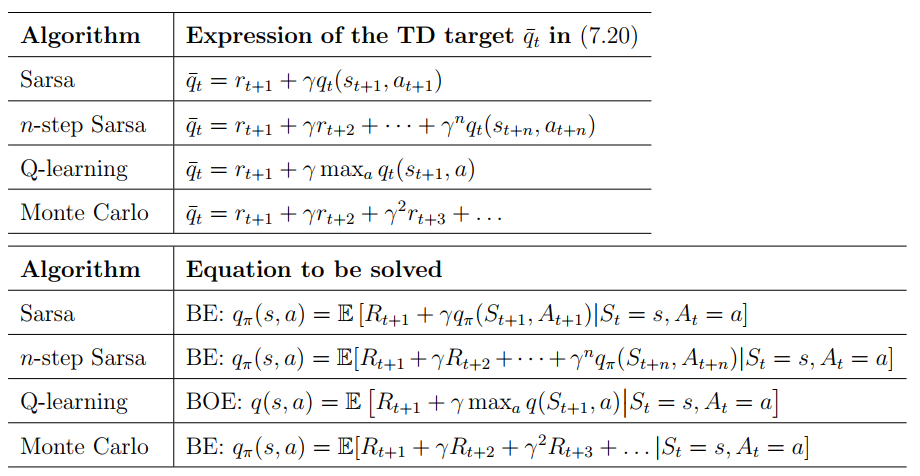
\includegraphics[width=0.90\textwidth]{image/td.png}
    \caption{TD algorithms}
    \label{fig:td}
\end{figure}


\section{Value Function Methods}
Instead of using table to represent the value function, which takes a lot of memory and does not generalize well at unknown state, we now introduce another way - 
using function estimation. In particular, the objective function is:
\begin{equation} \label{eq:obj_value_func}
    J(w) = \mathbb E \big [ (V^{\pi}(S) - \hat v(S, w))^2 \big ]
\end{equation}

We can use a uniform distribution as the distribution of $S$, but it does not consider the Markov process property. So we use \textbf{stationary distribution},
the long-term behavior, after sufficiently long period, every state will have its stationary probability. Let $\{ d_{\pi}(s) \}_{s \in \mathcal S}$ denote 
the stationary distribution of the Markov process under policy $\pi$. The objective is now:
\begin{equation}
    J(w) = \sum_{s \in \mathcal S} d_{\pi}(s) (V^{\pi}(S) - \hat v(S, w))^2
\end{equation}

\begin{definition}[Stationary Distribution]
    The probability of the agent transitioning from $s_i$ to $s_j$ using exactly $k$ steps is denoted as
    \[ p_{ij}^k = \Pr(S_{t_k} = j \mid S_{t_0} = i) \]
    by the definition of $P_{\pi}$, we have
    \[ [P_{\pi}]_{ij} = p_{ij}^{(1)} \]
    which means $[P_{\pi}]_{ij}$ is the probability of transitioning from $s_i$ to $s_j$ using a
single step. Second, consider $P^2_{\pi}$:
    \[ [P^2_{\pi}]_{ij} = [P_{\pi}P_{\pi}]_{ij} = \sum_{q=1}^n [P_{\pi}]_{iq}[P_{\pi}]_{qj} = p_{ij}^{(2)} \]
    In the same manner:
    \[ [P^n_{\pi}]_{ij} = p_{ij}^{(n)} \]
    Let $d_0 \in \mathcal R^n $ be a vector representing the probability distribution of the states at
the initial time step. Then 
    \begin{equation}
        d_k(s_i) = \sum_{j=1}^n d_0(s_j) [P^k_{\pi}]_{ji}, i = 1, 2, \ldots
    \end{equation}
    The matrix form is:
    \[ d_k^T = d_0^T P_{\pi}^k \]
    When we consider the long-term behavior of the Markov process, it holds under certain conditions that
    \[ \lim_{k \rightarrow \infty} P_{\pi}^k = \mathbf 1_n d_{\pi}^T \]
    $\mathbf 1_n d_{\pi}^T$ is a constant matrix with all its rows equal to $d_{\pi}^T$, 
    so
    \begin{equation} \label{eq:limiting_distribution}
        \lim_{k \rightarrow \infty} d_k^T = d_0^T \lim_{k \rightarrow \infty} P_{\pi}^k = d_0^T \mathbf 1_n d_{\pi}^T = d_{\pi}^T
    \end{equation}
    this means that the state distribution converges to a constant value $d_{\pi}$, which is called the limiting distribution, it is 
    independent of initial distribution $d_0$.

    The value of $d_{\pi}$ is by taking limit of $ d_k^T = d_{k-1}^T P_{\pi}$, where we will get
    \begin{equation} \label{eq:stationary_distribution}
        d_{\pi}^T = d_{\pi}^T P_{\pi}
    \end{equation}
    As a result, it is the left eigenvector of $P_{\pi}$ associated with eigenvalue 1.

    The solution of \ref{eq:stationary_distribution} is usually called a stationary distribution, whereas the distribution
in \ref{eq:limiting_distribution} is usually called the limiting distribution. Note that \ref{eq:limiting_distribution} implies \ref{eq:stationary_distribution}, 
but the converse may not be true. 

    \begin{itemize}
        \item State $s_j$ is said to be \mydefination{accessible} from $s_i$ f there exists a finite integer $k$
so that $[P^k_{\pi}]_{ij} > 0$.
        \item If two states $s_i$ and $s_j$ are mutually accessible, then the two states are said to \mydefination{communicate}.
        \item A Markov process is called \mydefination{irreducible} if all of its states communicate with each other. $k$ maybe different for different $i,j$.
        \item A Markov process is called \mydefination{regular} if there exists $k \geq 1$, such that $[P^k_{\pi}]_{ij} > 0, \forall i, j$. Regular Markov process
        is also irreducible, but the inverse is not. However, if a irreducible one exists $i$ such that $[P_{\pi}]_{ij} > 0$, then it is also regular. Moreover, 
        if $P^{k}_{\pi} > 0$, then for any $k \geq k'$, $P^{k'}_{\pi} > 0$.
    \end{itemize}
\end{definition}

We can use gradient descent to minimize the $J(w)$:
\[
\begin{array}{lll}
    \nabla_{w}J(w_{k})&=&\nabla_{w}\mathbb{E}[(v_{\pi}(S)-\hat{v}(S,w_{k}))^{2}] \\ 
    &=& \mathbb{E}[ \nabla_{w} (v_{\pi}(S)-\hat{v}(S,w_{k}))^{2} ] \\
    &=& 2\mathbb{E}[(v_{\pi}(S)-\hat{v}(S,w_{k}))(-\nabla_{w}\hat{v}(S,w_{k}))]\\ 
    &=& -2\mathbb{E}[(v_{\pi}(S)-\hat{v}(S,w_{k}))\nabla_{w}\hat{v}(S,w_{k})]
\end{array}
\]
therefore the algorithm is:
\begin{equation}
    w_{k+1}=w_{k}+2\alpha_{k}\mathbb{E}[(v_{\pi}(S)-\hat{v}(S,w_{k}))\nabla_{w}\hat{v}(S,w_{k})]
\end{equation}
with the stochastic replacement, and coefficient 2 merge into $\alpha_k$ without loss of generality, we get:
\begin{equation}
    w_{t+1}=w_{t}+\alpha_{t}\bigl(v_{\pi}(s_{t})-\hat{v}(s_{t},w_{t})\bigr)\nabla_{w}\hat{v}(s_{t},w_{t})
\end{equation}

Now we need to replace $v_{\pi}$, either with Monte Carlo:
\[ w_{t+1}=w_{t}+\alpha_{t}(g_{t}-\hat{v}(s_{t},w_{t}))\nabla_{w}\hat{v}(s_{t},w_{t}) \]
or with TD
\begin{equation} \label{eq:td_value_func}
    w_{t+1}=w_{t}+\alpha_{t}\left[r_{t+1}+\gamma\hat{v}(s_{t+1},w_{t})-\hat{v}(s_{t},w_{t})\right]\nabla_{w}\hat{v}(s_{t},w_{t}) 
\end{equation}

    \textbf{Tabular TD learning is a special case of TD-Linear}.

    However, \ref{eq:td_value_func} does not really solve \ref{eq:obj_value_func}, so we need to explain it rigorously. We first consider deterministic
algorithm:
\begin{equation}
    w_{t+1}=w_{t}+\alpha_{t}\mathbb{E}\biggl[(r_{t+1}+\gamma\phi^{T}(s_{t+1})w_{t}-\phi^{T}(s_{t})w_{t})\phi(s_{t})\biggr]
\end{equation}
then we will show \ref{eq:td_value_func} is the SGD implementation of it. Let 
\[
\Phi=\left[
    \begin{array}{c}{{\vdots}}\\ {{\phi^{T}(s)}}\\ {{\vdots}}
    \end{array}\right]\in\mathbb{R}^{n\times m},
\quad D=\left[
    \begin{array}{ccc}{{\ddots}}&{{}}\\ {{}}&{{d_{\pi}(s)}}&{{}}\\ {{}}&{{}}&{{\ddots}}\\
    \end{array}\right]\in\mathbb{R}^{n\times n}
\]

\begin{lemma} \label{lemma:td_value_func_rep}
    The expectation in \ref{eq:td_value_func} can be rewritten as
    \[ \mathbb{E}\Big[\big(r_{t+1}+\gamma\phi^{T}(s_{t+1})w_{t}-\phi^{T}(s_{t})w_{t}\big)\phi(s_{t})\Big]=b-A w_{t} \]
    where
    \begin{align*}
        A &\doteq \Phi^{T}D(I-\gamma P_{\pi})\Phi\in\mathbb{R}^{m\times m} \\ 
        b &\doteq \Phi^{T}D r_{\pi}\in\mathbb{R}^{m}.
    \end{align*}
    and $s_t$ is assumed to obey the stationary distribution $d_{\pi}$.
\end{lemma}

Then \ref{eq:td_value_func} can be rewritten as $w_{t+1}=w_{t}+\alpha_{t}(b-A w_{t})$, and it converges to $w^{\star}=A^{-1}b$, since 
$A$ is invertible and positive definite. Moreover, in the tabular case, as $n = |\mathcal S|$ and $\phi(s)=[0,\cdot\cdot\cdot,1,\cdot\cdot\cdot,0]^{T}$,
we will get $w^{*}\ =A^{-1}b\ =v_{\pi}$. These statements' proof please refer to the book section 8.2.

Then we show TD learning algorithm \ref{eq:td_value_func} minimizes the projected Bellman error. 
\ref{eq:obj_value_func} can be written in vector form as $J(w) = \| \hat v(w) - v_{\pi} \|_D^2$, where $\| x \|_D^2 = x^T D x = \| D^{1/2}x \|_2^2$, $D$ is 
given above. But this one has the true state value, so now we introduce Bellman error
\begin{equation} \label{eq:Bellman_error}
    J_{BE}(w) = \| \hat v(w) - (r_{\pi} + \gamma P_{\pi} \hat v(w)) \|_D^2 = \| \hat v(w) - T_{\pi} (\hat v(w)) \|_D^2
\end{equation}
where $T_{\pi}(x) = r_{\pi} + \gamma P_{\pi} x$ is the Bellman operator.

We can see this error may not be minimized to zero due to the limited approximation ability of the approximator. By contrast, an objective function
that can be minimized to zero is the projected Bellman error
\begin{equation} \label{eq:projected_Bellman_error}
    J_{PBE}(w) = \| \hat v(w) - MT_{\pi} (\hat v(w)) \|_D^2
\end{equation}
where $M \in \mathbb R^{n \times n}$ is the orthogonal projection matrix that geometrically projects any vector onto the space of all approximations.
We can show that $M=\Phi(\Phi^{T}D\Phi)^{-1}\Phi^{T}D\in\mathbb{R}^{n\times n}$ is the projection matrix that geometrically projects any vector onto 
the range space $\Phi$. Since $\hat v(w)$ is in the range space of $\Phi$, we can always find a value of w that can minimize
$J_{PBE}(w)$ to zero, it can be proven it is $w^{\star}=A^{-1}b$.

We can show that in linear case the bound of the error
\[ \|{\hat{v}}(w^{*})-v_{\pi}\|_{D}=
\|\Phi w^{*}-v_{\pi}\|_{D}\leq{\frac{1}{1-\gamma}}\operatorname*{min}_{w}\|{\hat{v}}(w)-v_{\pi}\|_{D}=
{\frac{1}{1-\gamma}}\operatorname*{min}_{w}\sqrt{J_{E}(w)} \]

Next we introduce \mydefination{least-squares} TD (LSTD), we can write $A$ and $b$ as (in proof of \ref{lemma:td_value_func_rep})
\begin{align*}
    A &= \mathbb{E}\left[\phi(s_{t})\left(\phi(s_{t})-\gamma\phi(s_{t+1})\right)^{T}\right], \\ 
    b &= \mathbb{E}\left[r_{t+1}\phi(s_{t})\right].
\end{align*}

The idea of LSTD is simple: if we can use random samples to directly obtain the estimates of $A$ and $b$, then the optimal parameter can be directly estimated.
In particular, given a trajectory $(s_0, r_1, s_1, \ldots)$ under $\pi$, we have
\begin{align}
    \hat{A}_{t} &= \sum_{k=0}^{t-1}\phi(s_{k})\left(\phi(s_{k})-\gamma\phi(s_{k+1})\right)^{T}, \\ 
    \hat{b}_{t} &= \sum_{k=0}^{t-1}r_{k+1}\phi(s_{k}).
\end{align}
we omitted $1 / t$, because it does not change the result that $w_{t}=\hat{A}_{t}^{-1}\hat{b}_{t}$.

The advantage of LSTD is that it uses experience samples more efficiently and converges faster than the TD method. 

The disadvantages of LSTD are as follows. First, it can only estimate state values. Moreover, while the TD algorithm allows nonlinear approximators, LSTD
does not. Second, the computational cost of LSTD is higher than that of TD since LSTD as we need to calculate inverse (but we can introduce a iterative algorithm
).

Now, all we talked in this section evaluate value function, but what about action values? We can modify \ref{eq:td_value_func}
\begin{equation} \label{eq:td_action_func}
    w_{t+1}=w_{t}+\alpha_{t}\Bigl[r_{t+1}+\gamma\hat{q}(s_{t+1},a_{t+1},w_{t})-\hat{q}(s_{t},a_{t},w_{t})\Bigr]\nabla_{w}\hat{q}(s_{t},a_{t},w_{t})
\end{equation}

\vspace{\baselineskip}

\begin{algorithm}[H]
\caption{Sarsa with function approximation}
\KwIn{Initial policy $\pi_0$, initial parameter $w_0$}
\KwOut{Learn an optimal policy that can lead the agent to the target state from an initial state $s_0$}

\ForEach{episode}{
    Generate $a_0$ at $s_0$ following $\pi_0(s_0)$ \\
    \While{$s_t (t = 0, 1, 2, \ldots) \neq s_{target}$}{
        Collect $(r_{t+1}, s_{t+1}, a_{t+1})$ given $(s_t, a_t)$, last one by following $\pi_t(s_{t+1})$, other by interacting with enviroment \\
        $w_{t+1}=w_{t}+\alpha_{t}\Bigl[r_{t+1}+\gamma\hat{q}(s_{t+1},a_{t+1},w_{t})-\hat{q}(s_{t},a_{t},w_{t})\Bigr]\nabla_{w}\hat{q}(s_{t},a_{t},w_{t})$ \\
        $\pi_{t+1}(a|s_t) \gets \begin{cases}
        1 - \frac{\epsilon}{|\mathcal A(s)|}(|\mathcal A(s)| - 1) & a = a^* = \arg\max_a q_{t+1}(s_t, a) \\
        \frac{\epsilon}{|\mathcal A(s)|} & a \neq a^*.
        \end{cases}$ \\
        $s_t \gets s_{t+1}, a_t \gets a_{t+1}$
    }
}
\end{algorithm}

\vspace{\baselineskip}

We can also modify Q-learning
\begin{equation}  \label{eq:td_action_func_q}
    w_{t+1}=w_{t}+\alpha_{t}\Bigl[r_{t+1}+\gamma\operatorname*{max}_{a\in A(s_{t+1})}\hat{q}(s_{t+1},a,w_{t})
    -\hat{q}(s_{t},a_{t},w_{t})\Bigr]\nabla_{w}\hat{q}(s_{t},a_{t},w_{t})
\end{equation}
again we can implement a on-policy or off-policy version.

Lastly, in this section we introduce \mydefination{Deep Q-learning} (DQN), the objective function is 
\begin{equation}
    J=\mathbb{E}\left[\left(R+\gamma\operatorname*{max}_{a\in A(S^{\prime})}{\hat{q}}(S^{\prime},a,w)-{\hat{q}}(S,A,w)\right)^{2}\right]
\end{equation}

This objective function can be viewed as the squared Bellman optimality error. That is because
\[
    q(s, a) = \mathbb{E} \left [ R_{t+1}+\gamma \max_{a\in A(S_{t+1})}q(S_{t+1},a) \mid S_{t}=s,A_{t}=a \right ]
\]
is the Bellman optimality equation (see last section).

For the sake of simplicity, it is assumed that the value of $w$ in $\gamma \max_{a\in A(S_{t+1})}q(S_{t+1},a)$ is fixed (for a short period of time)
so the calculation of the gradient becomes much easier. Let  
\[
    J=\mathbb{E}\left[\left(R+\gamma\operatorname*{max}_{a\in A(S^{\prime})}{\hat{q}}(S^{\prime},a,w_{T})-{\hat{q}}(S,A,w)\right)^{2}\right]
\]
where $w_{T}$ is the target network’s parameter which is fixed. Then the gradient is:
\begin{equation}
    \nabla_{w}J=-\mathbb{E}\left[
        \left(R+\gamma\operatorname*{max}_{a\in A(S^{\prime})}{\hat{q}}(S^{\prime},a,w_{T})-{\hat{q}}(S,A,w)\right)\nabla_{w}{\hat{q}}(S,A,w)
        \right]
\end{equation}

We need to pay attention that:
\begin{itemize}
    \item The first technique is to use two networks, a main network and a target network, as mentioned when we calculate the gradient, 
    let $w$ and $w_{T}$ denote the parameters of the main and target networks, respectively. They are initially set to the same value.
    The main network is updated in every iteration. By contrast, the target network is set to be the same as the main network every certain number of 
    iterations to satisfy the assumption that wT is fixed when calculating the gradient. 
    \item One notable difference between deep and nondeep reinforcement learning algorithms is that a mini-batch of samples to used to train a network in 
    DQN instead of using a single sample to update the main network.
    \item Let $(s, a, r, s')$ be an experience sample and $\mathcal B\doteq\{(s,a,r,s^{\prime})\}$ the \mydefination{replay buffer}. Every time we update the main 
    network, we can draw a mini-batch of experience samples from the replay buffer. The draw of samples, or called experience replay, \textbf{should follow 
    a uniform distribution}. The state-action samples may not be uniformly distributed in practice since they are generated as a sequence by the
behavior policy. It is necessary to break the correlation between the samples in the sequence to satisfy the assumption of uniform distribution. To do this, we can use
the experience replay technique by uniformly drawing samples from the replay buffer. A benefit of experience replay is that each experience sample may be used multiple
times, which can increase the data efficiency.
\end{itemize}

\vspace{\baselineskip}

\begin{algorithm}[H]
\caption{Deep Q-learning (off-policy version)}
\KwIn{A main network and a target network with the same initial parameter.}
\KwOut{Learn an optimal target network to approximate the optimal action values from
the experience samples generated by a given behavior policy $\pi_b$}

\Begin{
    Store the experience samples generated by $\pi_b$ in a replay buffer $\mathcal B\doteq\{(s,a,r,s^{\prime})\}$ \\
    \ForEach{iteration}{
        Uniformly draw a mini-batch of samples from $\mathcal B$ \\
        \ForEach{sample $(s_i, a_i, r_i, s_i')$}{
            $y_i \doteq r_i + \gamma \mathrm{max}_{a\in A(s^{\prime}_i)} \hat{q}(s^{\prime}_i,a,w_{T})$ \\
        }
        Update the main network to minimize $(y_{T}-\hat{q}(s,a,w))^{2}$ using the mini-batch of samples, for example, 
        $L(w) = \frac{1}{n} \sum_{i=1}^N (y_i - \hat q (s_i, a_i, w))^2$.
    }
    Set $w_T = w$ every $C$ iteration
}
\end{algorithm}

\vspace{\baselineskip}


\section{Policy Gradient Methods}
First, how to define optimal policies? When represented as a table, a policy is defined
as optimal if it can maximize \textbf{every state value}. When represented by a function, a
policy is defined as optimal if it can maximize certain \textbf{scalar metrics}.

We now introduce some metrics
\begin{definition}[Average State Value]
    Or average value, is defined as $\bar{v}_{\pi}=\sum_{s\in{\cal S}}d(s)v_{\pi}(s)$, where $d(s)$ is the weight
    of the state, It satisfles $d(s)\geq0$ for any $s\in S$ and $\sum_{s\in S}d(s)=1$. So we can interprete it as the probability distribution, so 
    $\bar{v}_{\pi}=\mathbb{E}_{S\sim d}[v_{\pi}(S)]$.

    Then how can we select $d$, we can choose it independent (we use $d_0$ and $\bar v_{\pi}^0$ as the notation) or dependent of policy (the stationary 
    distribution). Our ultimate goal is to find an optimal policy to maximize $\bar{v}_{\pi}$. It is the same as 
    \[ J(\theta)=\lim_{n\rightarrow\infty}\mathbb{E}\left[\sum_{t=0}^{n}\gamma^{t}R_{t+1}\right]=\mathbb{E}\left[\sum_{t=0}^{\infty}\gamma^{t}R_{t+1}\right] \]
    because
    \begin{align*}
        \mathbb{E}\left[\sum_{t=0}^{\infty}\gamma^{t}R_{t+1}\right] &= \sum_{s \in \mathcal S}d(s) \mathbb{E}\left[\sum_{t=0}^{\infty}\gamma^{t}R_{t+1} \mid S_0 = s \right] \\
        &= \sum_{s \in \mathcal S}d(s) v_{\pi}(s) \\
        &= \bar v_{\pi}(s)
    \end{align*}
    with the matrix form we have
    \[ \bar v_{\pi}(s) = d^T v_{\pi}(s) \]
\end{definition}

\begin{definition}[Average Reward]
    Or called average one-step reward, it is defined as
    \begin{align*}
        \bar{r}_{\pi} &\doteq \sum_{s\in{\cal S}}d_{\pi}(s)r_{\pi}(s) \\
        &= \mathbb E_{S\sim d_{\pi}}[r_{\pi}({S})]
    \end{align*}
    where $r_{\pi}(s)\doteq\sum_{a\in A}\pi(a|s,\theta)r(s,a)=\mathbb{E}_{A \in \pi(s,\theta)}[r(s,A)|s]$ is the expectation of the immediate rewards.
    Here $r(s,a)\doteq\mathbb{E}[R|s,a]=\sum_{r}r p(r|s,a)$.

    $\bar r_{\pi}$ is equivalent to
    \[ J(\theta)=\operatorname*{lim}_{n\rightarrow\infty}\frac{1}{n}  \mathbb E \left[\sum_{t=0}^{n-1}R_{t+1}\right] \]
    and
    \[ \bar{r}_{\pi}=\sum_{s\in S}d_{\pi}(s)r_{\pi}(s)=d_{\pi}^{T}r_{\pi} \]
\end{definition}

\begin{table}[ht]
\centering
\caption{Summary of the different but equivalent expressions of $\bar{v}_{\pi}$ and $\bar r_{\pi}$}
\begin{tabular}{cccc}
\toprule
Metric & Expression 1 & Expression 2 & Expression 3 \\
\midrule
$\bar{v}_{\pi}$ & $\sum_{s\in{\cal S}}d(s)v_{\pi}(s)$       & $\mathbb{E}_{S\sim d}[v_{\pi}(S)]$        & $\lim_{n\rightarrow\infty}\mathbb{E} \big [ \sum_{t=0}^{n}\gamma^{t}R_{t+1} \big ]$ \\
\midrule
$\bar r_{\pi}$  & $\sum_{s\in{\cal S}}d_{\pi}(s)r_{\pi}(s)$ & $\mathbb E_{S\sim d_{\pi}}[r_{\pi}({S})]$ & $\operatorname*{lim}_{n\rightarrow\infty}\frac{1}{n} \mathbb E \left[\sum_{t=0}^{n-1}R_{t+1}\right]$ \\
\bottomrule
\end{tabular}
\end{table}

\begin{theorem}[Policy gradient theorem]
    The gradient of $J(\theta)$ is
    \begin{equation}
        \nabla_{\theta}J(\theta)=\sum_{s\in{\mathcal{S}}}\eta(s)\sum_{a\in A}\nabla_{\theta}\pi(a|s,\theta)q_{\pi}(s,a)
    \end{equation}
    where $\eta$ is a state distribution and $\nabla_{\theta}\pi$ is the gradient of $\pi$ with respect to $\theta$. It has a compact form
    \begin{equation}
        \nabla_{\theta}J(\theta)=\mathbb{E}_{S\sim\eta,A\sim\pi(S,\theta)}\left[\nabla_{\theta}\ln\pi(A|S,\theta)q_{\pi}(S,A)\right]
    \end{equation}
    we can use softmax to make sure $\pi(a | s,\theta) \in (0, 1), \forall s \in \mathcal S$
    \begin{equation}
        \pi(a|s,\theta)=\frac{e^{h(s,a,\theta)}}{\sum_{a^{\prime}\in A}e^{h(s,a^{\prime},\theta)}},\quad a\in\mathcal{A}
    \end{equation}
    and in this sense the policy is exploratory.
\end{theorem}

\begin{lemma}
    \begin{equation}
        \bar{r}_{\pi}=(1-\gamma)\bar{v}_{\pi}
    \end{equation}
\end{lemma}

\begin{proof}
    Since $v_{\pi}=r_{\pi}+\gamma P_{\pi}v_{\pi}$, multiply $d_{\pi}^T$ on both side, we get
    \[ \bar{v}_{\pi}=\bar{\tau}_{\pi}+\gamma d_{\pi}^{T}{P}_{\pi}v_{\pi}=\bar{r}_{\pi}+\gamma d_{\pi}^{T}v_{\pi}=\bar{\tau}_{\pi}+\gamma\bar{v}_{\pi} \]
\end{proof}

\begin{lemma} \label{lemma:gradient_of_value_function}
    In the discounted case, it holds for any $s \in \mathcal S$ that
    \begin{equation} \label{eq:gradient_v_pi}
        \nabla_{\theta}v_{\pi}(s)=\sum_{s^{\prime}\in{\mathcal{S}}}\Pr_{\pi}(s^{\prime}|s)\sum_{a\in A}\nabla_{\theta}\pi(a|s^{\prime},\theta)q_{\pi}(s^{\prime},a)
    \end{equation}
    where
    \[
        \Pr_{\pi}(s^{\prime}|s)\doteq\sum_{k=0}^{\infty}\gamma^{k}[P_{\pi}^{k}]_{s s^{\prime}}=\big[(I_{n}-\gamma P_{\pi})^{-1}\big]_{s s^{\prime}}
    \]
    is the discounted total probability of transitioning from $s$ to $s'$ under policy $\pi$. Here $[\cdot]_{ss'}$ denotes the entry in the $s$th row and 
    $s'$th column, $k$ means exactly $k$ steps.
\end{lemma}

\begin{proof}
    \begin{equation}
        \begin{array}{lll}
            \nabla_{\theta}v_{\pi}(s) &=& \nabla_{\theta}\big [\sum_{a\in A}\pi(a|s,\theta)q_{\pi}(s,a)\big ] \\
            &=& \sum_{a\in A}\big [ \nabla_{\theta}\pi(a | s,\theta)q_{\pi}(s,a)+\pi (a | s,\theta)\nabla_{\theta}q_{\pi}(s,a)\big ]
        \end{array}
    \end{equation}
    where 
    \[
        q_{\pi}(s,a)=r(s,a)+\gamma\sum_{s^{\prime}\in{\mathcal{S}}}p(s^{\prime}|s,a)v_{\pi}(s^{\prime})
    \]
    since $r(s,a)=\sum_{r}r p(r|s,a)$ is independent of $\theta$
    \[
    \nabla_{\theta}q_{\pi}(s,a)=0+\gamma\sum_{s^{\prime}\in S}p(s^{\prime}|s,a)\nabla_{\theta}v_{\pi}(s^{\prime})
    \]
    substitute this into the first equation we have
    \begin{equation}
        \begin{array}{lll}
            \nabla_{\theta}v_{\pi}(s) &=& \sum_{a\in A}\left[\nabla_{\theta}\pi(a|s,\theta)q_{\pi}(s,a)+\pi(a|s,\theta)\gamma\sum_{s^{\prime}\in S}p(s^{\prime}|s,a)\nabla_{\theta}v_{\pi}(s^{\prime})\right] \\
            &=& \sum_{a\in A}\nabla_{\theta}\pi(a|s,\theta)q_{\pi}(s,a)+\gamma\sum_{a\in A}\pi(a|s,\theta)\sum_{s^{\prime}\in S}p(s^{\prime}|s,a)\nabla_{\theta}v_{\pi}(s^{\prime})
        \end{array}
    \end{equation}
    One way to calculate it is to use the \textbf{unrolling technique}, we use another way based on the matrix-vector form, let
    \[
        u(s)\doteq\sum_{a\in\mathcal{A}}\nabla_{\theta}\pi(a|s,\theta)q_{\pi}(s,a)
    \]
    Since 
    \[
        \sum_{a\in A}\pi(a|s,\theta)\sum_{s^{\prime}\in{\cal S}}p(s^{\prime}|s,a)\nabla_{\theta}v_{\pi}(s^{\prime})
        =\sum_{s^{\prime}\in{\cal S}}p(s^{\prime}|s)\nabla_{\theta}v_{\pi}(s^{\prime})
        =\sum_{s^{\prime}\in{\cal S}}[P_{\pi}]_{s s^{\prime}}\nabla_{\theta}v_{\pi}(s^{\prime})
    \]
    the matrix form is
    \[
        \underbrace{
            \begin{bmatrix}
                \vdots \\ \nabla_{\theta}v_{\pi}(s) \\ \vdots
            \end{bmatrix}
        }_{\nabla_{\theta}v_{\pi} \in \mathbb R^{mn}}
        =
        \underbrace{
            \begin{bmatrix}
                \vdots \\ u(s) \\ \vdots
            \end{bmatrix}
        }_{u \in \mathbb R^{mn}}
        +
        \gamma(P_{\pi}\otimes I_{m})
        \underbrace{
            \begin{bmatrix}
                \vdots \\ \nabla_{\theta}v_{\pi}(s') \\ \vdots
            \end{bmatrix}
        }_{\nabla_{\theta}v_{\pi} \in \mathbb R^{mn}}
    \]
    which can be written concisely as
    \[
        \nabla_{\theta}v_{\pi}=u+\gamma(P_{\pi}\otimes I_{m})\nabla_{\theta}v_{\pi}
    \]
    here $n = |\mathcal S|$ and $m$ is the dimension of the parameter vector $\theta$.
    Then
    \begin{equation}
        \begin{array}{lll}
            \nabla_{\theta}v_{\pi} &=& (I_{n m}-\gamma P_{\pi}\otimes I_{m})^{-1}u \\
            &=& (I_{n}\otimes I_{m}-\gamma P_{\pi}\otimes I_{m})^{-1}u \\
            &=& \left[(I_{n}-\gamma P_{\pi})^{-1}\otimes I_{m}\right]u
        \end{array}
    \end{equation}
    from this we get
    \begin{equation}
        \begin{array}{lll}
            \nabla_{\theta}v_{\pi}(s) &=& \sum_{s^{\prime}\in{\mathcal{S}}}\left[(I_{n}-\gamma P_{\pi})^{-1}\right]_{s s^{\prime}}u(s^{\prime}) \\
            &=& \sum_{s^{\prime}\in{\mathcal{S}}}\left[(I_{n}-\gamma P_{\pi})^{-1}\right]_{s s^{\prime}}\sum_{a\in A}\nabla_{\theta}\pi(a|s^{\prime},\theta)q_{\pi}(s^{\prime},a)
        \end{array}
    \end{equation}
    since $(I_{n}-\gamma P_{\pi})^{-1}=I+\gamma P_{\pi}+\gamma^{2}P_{\pi}^{2}+\dots$
    \[
        [(I_{n}-\gamma P_{\pi})^{-1}]_{s s^{\prime}}=[I]_{s s^{\prime}}+\gamma[P_{\pi}]_{s s^{\prime}}+\gamma^{2}[P_{\pi}^{2}]_{s s^{\prime}}+\cdots=\sum_{k=0}^{\infty}\gamma^{k}[P_{\pi}^{k}]_{s s^{\prime}}
    \]
    denote $[(I_{n}-\gamma P_{\pi})^{-1}]_{s s^{\prime}} \doteq \Pr_{\pi}(s' | s)$, we get \ref{eq:gradient_v_pi}.
\end{proof}

\begin{theorem}[Gradient of $\bar v_{\pi}^0$ in the discounted case]
    In the discounted case where $\gamma \in (0, 1)$, the gradient of $\bar v_{\pi}^0$ is
    \[
        \nabla_{\theta}\bar{v}_{\pi}^{0}=\mathbb{E}\big[\nabla_{\theta}\ln\pi(A|S,\theta)q_{\pi}(S,A)\big]
    \]
    where $S \sim \rho_{\pi}$ and $A \sim \pi(S, \theta)$, the state distribution is
    \begin{equation}
        \rho_{\pi}(s)=\sum_{s^{\prime}\in{\mathcal{S}}}d_{0}(s^{\prime})\Pr_{\pi}(s|s^{\prime}), \quad s\in{\mathcal{S}}
    \end{equation}
\end{theorem}

\begin{proof}
    Since $d_0(s)$ is independent of $\pi$, we have
    \[
        \nabla_{\theta}\bar{v}_{\pi}^{0}=\nabla_{\theta}\sum_{s\in{\cal S}}d_{0}(s)v_{\pi}(s)=\sum_{s\in{\cal S}}d_{0}(s)\nabla_{\theta}v_{\pi}(s)
    \]
    then
    \[
    \begin{aligned}
    \nabla_{\theta} \bar{v}_{\pi}^{0} 
    &= \sum_{s \in \mathcal{S}} d_0(s) \nabla_{\theta} v_{\pi}(s) \\
    &= \sum_{s \in \mathcal{S}} d_0(s) \sum_{s' \in \mathcal{S}} \Pr_{\pi}(s'|s) \sum_{a \in \mathcal{A}} \nabla_{\theta} \pi(a|s', \theta) q_{\pi}(s', a) \\
    &= \sum_{s' \in \mathcal{S}} \left( \sum_{s \in \mathcal{S}} d_0(s) \Pr_{\pi}(s'|s) \right) \sum_{a \in \mathcal{A}} \nabla_{\theta} \pi(a|s', \theta) q_{\pi}(s', a) \\
    &\doteq \sum_{s' \in \mathcal{S}} \rho_{\pi}(s') \sum_{a \in \mathcal{A}} \nabla_{\theta} \pi(a|s', \theta) q_{\pi}(s', a) \\
    &= \sum_{s \in \mathcal{S}} \rho_{\pi}(s) \sum_{a \in \mathcal{A}} \nabla_{\theta} \pi(a|s, \theta) q_{\pi}(s, a) \quad \text{(change $s'$ to $s$)} \\
    &= \sum_{s \in \mathcal{S}} \rho_{\pi}(s) \sum_{a \in \mathcal{A}} \pi(a|s, \theta) \nabla_{\theta} \ln \pi(a|s, \theta) q_{\pi}(s, a) \\
    &= \mathbb{E}\left[ \nabla_{\theta} \ln \pi(A|S, \theta) q_{\pi}(S, A) \right],
    \end{aligned}
    \]
\end{proof}

\begin{theorem}[Gradient of $\bar v_{\pi}$ and $\bar r_{\pi}$ in the discounted case]
    In the discounted case where $\gamma \in (0, 1)$, the gradient of $\bar v_{\pi}$ and $\bar r_{\pi}$ are
    \begin{equation}
        \nabla_{\theta}\bar{r}_{\pi}=(1-\gamma)\nabla_{\theta}\bar{v}_{\pi}
        \approx
        \sum_{s\in{\mathcal{S}}}d_{\pi}(s)\sum_{a\in A}\nabla_{\theta}\pi(a|s,\theta)q_{\pi}(s,a)
        =\mathbb{E}\left[\nabla_{\theta}\ln\pi(A|S,\theta)q_{\pi}(S,A)\right]
    \end{equation}
    Here, the approximation is more accurate when $\gamma$ is closer to 1.
\end{theorem}

\begin{proof}
    It follows from the definition of $\bar{v}_{\pi}$ that
    \[
    \begin{aligned}
        \nabla_{\theta} \bar{v}_{\pi} &= \nabla_{\theta} \sum_{s \in \mathcal{S}} d_{\pi}(s) v_{\pi}(s) \\
        &= \sum_{s \in \mathcal{S}} \nabla_{\theta} d_{\pi}(s) v_{\pi}(s) + \sum_{s \in \mathcal{S}} d_{\pi}(s) \nabla_{\theta} v_{\pi}(s).
    \end{aligned}
    \]

    This equation contains two terms. On the one hand, substituting the expression of $\nabla_{\theta} v_{\pi}$ given in (9.17) into the second term gives
    \[
    \begin{aligned}
        \sum_{s \in \mathcal{S}} d_{\pi}(s) \nabla_{\theta} v_{\pi}(s)
        &= \left( d_{\pi}^{\top} \otimes I_m \right) \nabla_{\theta} v_{\pi} \\
        &= \left( d_{\pi}^{\top} \otimes I_m \right) \left[ (I_n - \gamma P_{\pi})^{-1} \otimes I_m \right] u \\
        &= \left[ d_{\pi}^{\top} (I_n - \gamma P_{\pi})^{-1} \right] \otimes I_m u.
    \end{aligned}
    \]

    It is noted that
    \[
    d_{\pi}^{\top} (I_n - \gamma P_{\pi})^{-1} = \frac{1}{1 - \gamma} d_{\pi}^{\top},
    \]
    which can be easily verified by multiplying $(I_n - \gamma P_{\pi})$ on both sides of the equation. Therefore, the above becomes
    \[
    \begin{aligned}
        \sum_{s \in \mathcal{S}} d_{\pi}(s) \nabla_{\theta} v_{\pi}(s)
        &= \frac{1}{1 - \gamma} d_{\pi}^{\top} \otimes I_m u \\
        &= \frac{1}{1 - \gamma} \sum_{s \in \mathcal{S}} d_{\pi}(s) \sum_{a \in \mathcal{A}} \nabla_{\theta} \pi(a|s, \theta) q_{\pi}(s, a).
    \end{aligned}
    \]

    On the other hand, the first term of the earlier expression involves $\nabla_{\theta} d_{\pi}$. However, since the second term contains $\frac{1}{1 - \gamma}$, the second term becomes dominant, and the first term becomes negligible when $\gamma \to 1$. Therefore,
    \[
    \nabla_{\theta} \bar{v}_{\pi} \approx \frac{1}{1 - \gamma} \sum_{s \in \mathcal{S}} d_{\pi}(s) \sum_{a \in \mathcal{A}} \nabla_{\theta} \pi(a|s, \theta) q_{\pi}(s, a).
    \]

    Furthermore, it follows from $\bar{r}_{\pi} = (1 - \gamma) \bar{v}_{\pi}$ that
    \[
    \begin{aligned}
        \nabla_{\theta}\bar{r}_{\pi}=(1-\gamma)\nabla_{\theta}\bar{v}_{\pi} &\approx 
        \sum_{s\in{\mathcal{S}}}d_{\pi}(s)\sum_{a\in A}\nabla_{\theta}\pi(a|s,\theta)q_{\pi}(s,a) \\
        &= \sum_{s\in{\mathcal{S}}}d_{\pi}(s)\sum_{a\in A} \pi(a|s,\theta) \nabla_{\theta}\ln \pi(a|s,\theta)q_{\pi}(s,a) \\
        &= \mathbb{E}\left[\nabla_{\theta}\ln\pi(A|S,\theta)q_{\pi}(S,A)\right]
    \end{aligned}
    \]
\end{proof}

For the undiscounted case, it is necessary to redefine state and action values since they maybe diverge
\[
    v_{\pi}(s)\doteq\mathbb{E} \big [(R_{t+1}-{\bar{r}}_{\pi})+(R_{t+2}-{\bar{r}}_{\pi})+(R_{t+3}-{\bar{r}}_{\pi})+\dots | S_{t}=s \big]
\]

\[
    q_{\pi}(s,a)\doteq\mathbb{E} \big [(R_{t+1}-{\bar{r}}_{\pi})+(R_{t+2}-{\bar{r}}_{\pi})+(R_{t+3}-{\bar{r}}_{\pi})+\dots | S_{t}=s,A_{t}=a \big ]
\]

It can be verified that the state value defined above satisfies the following Bellman-like equation
\begin{equation}
    v_{\pi}(s)=\sum_{a}\pi(a|s,\theta)\left[\sum_{r}p(r|s,a)(r-{\bar{r}}_{\pi})+\sum_{s^{\prime}}p(s^{\prime}|s,a)v_{\pi}(s^{\prime})\right]
\end{equation}
The matrix form is 
\[
    v_{\pi} = r_{\pi} - \bar r_{\pi}\mathbf 1_{n}\ +P_{\pi}v_{\pi}
\]
it is similar to the Bellman equation and it has a specific name called the \textbf{Poisson equation}.

\begin{theorem}[Solution of the Poisson equation]
    Let 
    \begin{equation}
        v_{\pi}^{\ast}=(I_{n}-P_{\pi}+{\bf 1}_{n}d_{\pi}^{T})^{-1}r_{\pi}
    \end{equation}
    Then, $v_{\pi}^{\ast}$ is a solution of the Poisson equation. Moreover, any solution of the
Poisson equation has the following form:
    \[ v_{\pi} = v_{\pi}^{\ast} + c \bf 1_n \]
\end{theorem}

Because of $c$, the value of $v_{\pi}$ is not unique, but $\bar r_{\pi}$ is
\[
\begin{array}{lll}
    \bar{r}_{\pi}{\bf1}_{n} &=& r_{\pi}+(P_{\pi}-I_{n})v_{\pi} \\ 
    \phantom{\qquad} &=& r_{\pi}+(P_{\pi}-I_{n})(v_{\pi}^{*}+c{\bf1}_{n}) \\ 
    \phantom{\qquad} &=& r_{\pi}+(P_{\pi}-I_{n})v_{\pi}^{*}.
\end{array}
\]

\begin{theorem}[Gradient of $\bar r_{\pi}$ in the undiscounted case]
    \begin{equation}
        \begin{aligned}
        \nabla_{\theta}\bar{r}_{\pi} &=\sum_{s\in{\mathcal{S}}}d_{\pi}(s)\sum_{a\in A}\nabla_{\theta}\pi(a|s,\theta)q_{\pi}(s,a) \\
        &= \mathbb{E}\left[\nabla_{\theta}\ln\pi(A|S,\theta)q_{\pi}(S,A)\right]
        \end{aligned}
    \end{equation}
\end{theorem}

We now introduce \mydefination{Monte Carlo policy gradient} (REINFORCE), gradient-ascent algorithm for maximizing $J(\theta)$ is
\begin{equation} \label{eq:policy_gradient}
    \begin{aligned}
        \theta_{t+1} &=\theta_{t}+\alpha\nabla_{\theta}J(\theta_{t}) \\
        &=\theta_{t}+\alpha\mathbb{E}\biggl[\nabla_{\theta}\ln\pi(A|S,\theta_{t})q_{\pi}(S,A)\biggr] \\
        &\rightarrow \quad \text{stochastic gradient} \\
        &= \theta_{t}+\alpha\nabla_{\theta}\ln\pi(a_{t}|s_{t},\theta_{t})q_{t}(s_{t},a_{t})
    \end{aligned}
\end{equation}
if $q_{t}(s_{t},a_{t})$ is obtained by Monte Carlo estimation, which is one of earliest and simplest policy gradient algorithms.

rewrite it 
\begin{equation}
    \theta_{t+1}=\theta_{t} +\alpha
    \underbrace{\left(\frac{q_{t}(s_{t},a_{t})}{\pi(a_{t}|s_{t},\theta_{t})}\right)}_{\beta_t}
    \nabla_{\theta}\pi(a_{t}|s_{t},\theta_{t})
    =\theta_{t} +\alpha \beta_t \nabla_{\theta}\pi(a_{t}|s_{t},\theta_{t})
\end{equation}

\begin{enumerate}
    \item If $\beta_t \geq 0$, the probability of choosing $(s_t, a_t)$ is enhanced.
    \item the algorithm can strike a balance between exploration and exploitation to a certain extent due to the expression of $\beta_t$.
    \item How to sample $S$, the distribution is long term behavior of $d_{\pi}$ or $\rho_{\pi}$.
    \item How to sample $A$, it should follow $\pi(A | S, \theta)$.
    \item Unfortunately, the ideal ways for sampling $S$ and $A$ are not strictly followed in practice
due to their low efficiency of sample usage.
\end{enumerate}

\vspace{\baselineskip}

\begin{algorithm}[H]
\caption{Policy Gradient by Monte Carlo (REINFORCE)}
\KwIn{Initial parameter $\theta$.}
\KwOut{Learn an optimal policy for maximizing $J(\theta)$.}

\ForEach{episode}{
    Generate an episode $\{s_0, a_0, r_1, \ldots, r_T\}$ following $\pi(\theta)$ \\
    \For{$t = 0, 1, \ldots, T-1$}{
        Value update: $q_{t}(s_{t},a_{t})=\sum_{k=t+1}^{T}\gamma_{s}^{k-t-1}r_{k}$ \\
        Policy update: $\theta\leftarrow\theta+\alpha\nabla_{\theta}\ln{{\pi}}(a_{t}|s_{t},\theta)q_{t}(s_{t},a_{t})$
    }
}
\end{algorithm}

\vspace{\baselineskip}



\section{Actor-Critic Methods}
Here, an ``actor" refers to a policy update step. The reason that it is called an actor is that the
actions are taken by following the policy. Here, an ``critic" refers to a value update step. It
is called a critic because it criticizes the actor by evaluating its corresponding values. From
another point of view, actor-critic methods are still policy gradient algorithms. 

If in \ref{eq:policy_gradient}, we use Monte Carlo method, then it is REINFORCE, if it uses TD to evaluate $q(s, a)$, then is is
\mydefination{actor-critic}.

\vspace{\baselineskip}

\begin{algorithm}[H]
\caption{The simplest actor-critic algorithm (QAC)}
\KwIn{Initial parameter $\theta_0$ and policy function $\pi(a | s, \theta_0)$. A value function $q(s, a, w_0)$, $\alpha_w, \alpha_{\theta} > 0$}
\KwOut{Learn an optimal policy for maximizing $J(\theta)$.}

\ForEach{time step $t$ in each episode}{
    Generate $a_t$ following $\pi(a, s_t, \theta_t)$, observe $r_{t+1}, s_{t+1}$ and then generate $a_{t+1}$ following $\pi(a, s_{t+1}, \theta_t)$ \\
    Actor (Policy update): $\theta_{t+1} \leftarrow \theta_t +\alpha_{\theta} \nabla_{\theta}\ln{{\pi}}(a_{t}|s_{t},\theta_t)q_{t}(s_{t},a_{t}, w_t)$ \\
    Critic (Value update): $w_{t+1}=w_{t}+\alpha_{w}[r_{t+1}+\gamma q(s_{t+1},a_{t+1},w_{t})-q(s_{t},a_{t},w_{t})]\nabla_{w}q(s_{t},a_{t},w_{t})$
}
\end{algorithm}

\vspace{\baselineskip}

We then introduce \mydefination{Advantage Actor-Critic} (A2C), the core idea of this algorithm
is to introduce a baseline to reduce estimation variance.

One interesting property of the policy gradient is that it is invariant to an additional
baseline
\begin{equation}
    \mathbb{E}_{S{\sim}\eta,A{\sim}\pi}\Bigl[\nabla_{\theta}\ln\pi(A|S,\theta_{t})q_{\pi}(S,A)\Bigr]=\mathbb{E}_{S{\sim}\eta,A{\sim}\pi}\Bigl[\nabla_{\theta}\ln\pi(A|S,\theta_{t})(q_{\pi}(S,A)-b(S)\Bigr]
\end{equation}
this holds if and only if
\[
    \mathbb{E}_{S\sim\eta,A\sim\pi}\Bigl[\nabla_{\theta}\ln\pi\bigl(A|S,\theta_{t}\bigr)b(S)\Bigr]=0
\]
this is valid because
\[
    \begin{aligned}
        \mathbb{E}_{S\sim\eta,A\sim\pi}\Bigl[\nabla_{\theta}\ln\pi\bigl(A|S,\theta_{t}\bigr)b(S)\Bigr]
        &= \sum_{s\in{\mathcal{A}}}\eta(s)\sum_{a\in{\mathcal{A}}}\pi(a|s,\theta_{t})\nabla_{\theta}\ln\pi(a|s,\theta_{t})b(s) \\
        &= \sum_{s\in{\cal S}}\eta(s)\sum_{a\in A}\nabla_{\theta}\pi(a|s,\theta_{t})b(s) \\
        &= \sum_{s\in{\mathcal{S}}}\eta(s)b(s)\sum_{a\in A}\nabla_{\theta}\pi(a|s,\theta_{t}) \\
        &= \sum_{s\in S}\eta(s)b(s)\nabla_{\theta}\sum_{a\in\mathcal{A}}\pi(a|s,\theta_{t}) \\
        &= \sum_{s\in{\mathcal{S}}}\eta(s)b(s)\nabla_{\theta}1=0
    \end{aligned}
\]

The baseline is useful because it can reduce the approximation variance when we use
samples to approximate the true gradient. In particular, let
\begin{equation}
    X(S,A) \doteq \nabla_{\theta}\ln\pi(A|S,\theta_{t})[q_{\pi}(S,A)-b(S)]
\end{equation}

Then, the true gradient is $\mathbb E [X(S,A)]$. In REINFORCE and QAC, we set $b = 0$, which is not guaranteed to be a good baseline.

In fact, the optimal baseline that minimizes $\text{var}(X)$ is (please refer to book box 10.1)
\begin{equation}
    b^{\ast}(s) = \frac{\mathbb{E}_{A\sim\pi}\left[||\nabla_{\theta}\ln\pi(A|s,\theta_{t})||^{2}q_{\pi}(s,A)\right]}
    {\mathbb{E}_{A \sim \pi}\left[||\nabla_{\theta}\ln\pi\left(A|S,\theta_{t}\right)||^{2}\right]}, \quad s \in \mathcal S
\end{equation}
but this is too complex, we use a suboptimal one:
\[
    b^{\dagger}(s)=\mathbb{E}_{A\sim\pi}[q_{\pi}(s,A)]=v_{\pi}(s),\quad s\in\mathcal{S}
\]
Interestingly, this suboptimal baseline is the state value.

The algorithm is then
\begin{equation}
    \begin{aligned}
        \theta_{t+1} &= \theta_t + \alpha \mathbb E \big [ \nabla_{\theta} \ln \pi(A|S,\theta_{t}) [q_{\pi}(S,A) - v_{\pi}(S)] \big ] \\
        &= \theta_t + \alpha \mathbb E \big [ \nabla_{\theta} \ln \pi(A|S,\theta_{t}) \delta_{\pi}(S,A) \big ] \\
        &\rightarrow \quad \text{stochastic version} \\
        &= \theta_{t}+\alpha\nabla_{\theta}\ln\pi(a_{t}|s_{t},\theta_{t})[q_{t}(s_{t},a_{t})-v_{t}(s_{t})] \\
        &= \theta_{t}+\alpha\nabla_{\theta}\ln\pi(a_{t}|s_{t},\theta_{t})\delta_{t}(s_{t},a_{t})
    \end{aligned}
\end{equation}

If $q_t(s_t, a_t)$ and $v_t(s_t)$ are estimated by Monte Carlo learning, this is
called REINFORCE with a baseline. If they are estimated by TD learning,
the algorithm is usually called advantage actor-critic (A2C).

\vspace{\baselineskip}

\begin{algorithm}[H]
\caption{Advantage actor-critic (A2C) or TD actor-critic}
\KwIn{Initial parameter $\theta_0$ and policy function $\pi(a | s, \theta_0)$. A value function $v(s, w_0)$, $\alpha_w, \alpha_{\theta} > 0$}
\KwOut{Learn an optimal policy for maximizing $J(\theta)$.}

\ForEach{time step $t$ in each episode}{
    Generate $a_t$ following $\pi(a, s_t, \theta_t)$, observe $r_{t+1}, s_{t+1}$ \\
    Advantage: $\delta_t = r_{t+1}+\gamma v_{t}(s_{t+1}, w_t)-v_{t}(s_{t}, w_t)$ \\
    Actor (Policy update): $\theta_{t+1} \leftarrow \theta_t +\alpha_{\theta} \delta_t \nabla_{\theta}\ln{{\pi}}(a_{t}|s_{t},\theta_t)$ \\
    Critic (Value update): $w_{t+1}=w_{t}+\alpha_{w} \delta_t \nabla_{w}v(s_{t},w_{t})$
}
\end{algorithm}

\vspace{\baselineskip}

It should be noted that the advantage function in this
implementation is approximated by the TD error
\[
    q_{t}(s_{t},a_{t})-v_{t}(s_{t})\approx r_{t+1}+\gamma v_{t}(s_{t+1})-v_{t}(s_{t})
\]
This approximation is reasonable because
\[
    q_{\pi}(s_{t},a_{t})-v_{\pi}(s_{t})=\mathbb{E}\left[R_{t+1}+\gamma v_{\pi}(S_{t+1})-v_{\pi}(S_{t})\vert S_{t}=s_{t},A_{t}=a_{t}\right]
\]
When we use the TD error, the algorithm may also be called TD actor-critic.

All the methods we talked above is on-policy, now we introduce off-policy one. But first we introduce \mydefination{Importance Sampling},
if $x$ is generated with $p_1$, we want use $p_0$ to evaluate expectation
\begin{equation}
    \mathbb{E}_{X\sim p_{0}}[X]=\sum_{x\in{\mathcal{X}}}p_{0}(x)x
    =\sum_{x\in{\mathcal{X}}}p_{1}(x) \underbrace{\frac{p_{0}(x)}{p_{1}(x)}}_{f(x)x}=\mathbb{E}_{X\sim p_{1}}[f(X)]
\end{equation}
and then
\begin{equation}
    \mathbb{E}_{X{\sim}p_{0}}[X]
    =\mathbb{E}_{X{\sim}p_{1}}[f(X)]\approx{\bar{f}}
    ={\frac{1}{n}}\sum_{i=1}^{n}f(x_{i})
    ={\frac{1}{n}}\sum_{i=1}^{n} \underbrace{\frac{p_0(x_i)}{p_1(x_i)}}_{\text{importance weight}} x_{i}.
\end{equation}

Suppose the behavior policy is $\beta$, than what we want to optimize is
\[
    J(\theta)=\sum_{s\in{\cal S}}d_{\beta}(s)v_{\pi}(s)=\mathbb{E}_{S \sim d_{\beta}}[v_{\pi}(s)]
\]

\begin{theorem}[Off-policy policy gradient theorem]
    In the discounted case, the gradient is
    \begin{equation}
        \nabla_{\theta}J(\theta)=
        \mathbb{E}_{S\sim\rho,A\sim\beta}{\Bigg[}
        \underbrace{\frac{\pi(A|S,\theta)}{\beta(A|S)}}_{\text{importance weight}}\,\nabla_{\theta}\ln\pi(A|S,\theta)q_{\pi}(S,A){\Bigg]}
    \end{equation}
    where the state distribution $\rho$ is
    \[
        \rho(s)\doteq\sum_{s^{\prime}\in{\cal S}}d_{\beta}(s^{\prime})\Pr_{\pi}(s|s^{\prime}),\quad s\in\cal{S}
    \]
    where
    \[
        \Pr_{\pi}(s|s^{\prime})=\sum_{k=0}^{\infty}\gamma^{k}[P_{\pi}^{k}]_{s^{\prime}s}=[(I-\gamma P_{\pi})^{-1}]_{s^{\prime}s}
    \]
\end{theorem}

\begin{proof}
    Since $d_{\beta}$ is independent of $\theta$, the gradient of $J(\theta)$ satisfies
    \begin{equation}
    \nabla_{\theta} J(\theta) = \nabla_{\theta} \sum_{s \in \mathcal{S}} d_{\beta}(s) v_{\pi}(s) = \sum_{s \in \mathcal{S}} d_{\beta}(s) \nabla_{\theta} v_{\pi}(s).
    \end{equation}

    According to Lemma \ref{lemma:gradient_of_value_function}, the expression of $\nabla_{\theta} v_{\pi}(s)$ is
    \begin{equation}
    \nabla_{\theta} v_{\pi}(s) = \sum_{s' \in \mathcal{S}} \text{Pr}_{\pi}(s'|s) \sum_{a \in \mathcal{A}} \nabla_{\theta} \pi(a|s', \theta) q_{\pi}(s', a)
    \end{equation}
    where $\text{Pr}_{\pi}(s'|s) \doteq \sum_{k=0}^{\infty} \gamma^k [P_{\pi}^k]_{ss'} = [(I_n - \gamma P_{\pi})^{-1}]_{ss'}$. Then we have

    \begin{align*}
    \nabla_{\theta} J(\theta) 
    = \sum_{s \in \mathcal{S}} d_{\beta}(s) \nabla_{\theta} v_{\pi}(s) 
    &= \sum_{s \in \mathcal{S}} d_{\beta}(s) \sum_{s' \in \mathcal{S}} \text{Pr}_{\pi}(s'|s) \sum_{a \in \mathcal{A}} \nabla_{\theta} \pi(a|s', \theta) q_{\pi}(s', a) \\
    &= \sum_{s' \in \mathcal{S}} \left( \sum_{s \in \mathcal{S}} d_{\beta}(s) \text{Pr}_{\pi}(s'|s) \right) \sum_{a \in \mathcal{A}} \nabla_{\theta} \pi(a|s', \theta) q_{\pi}(s', a) \\
    &\doteq \sum_{s' \in \mathcal{S}} \rho(s') \sum_{a \in \mathcal{A}} \nabla_{\theta} \pi(a|s', \theta) q_{\pi}(s', a) \\
    &= \sum_{s \in \mathcal{S}} \rho(s) \sum_{a \in \mathcal{A}} \nabla_{\theta} \pi(a|s, \theta) q_{\pi}(s, a) \quad \text{(change } s' \text{ to } s) \\
    &= \mathbb{E}_{S \sim \rho} \left[ \sum_{a \in \mathcal{A}} \nabla_{\theta} \pi(a|S, \theta) q_{\pi}(S, a) \right].
    \end{align*}

    By using the importance sampling technique, the above equation can be further rewritten as
    \begin{align*}
    \mathbb{E}_{S \sim \rho} \left[ \sum_{a \in \mathcal{A}} \nabla_{\theta} \pi(a|S, \theta) q_{\pi}(S, a) \right]
    &= \mathbb{E}_{S \sim \rho} \left[ \sum_{a \in \mathcal{A}} \beta(a|S) \frac{\pi(a|S, \theta)}{\beta(a|S)} \frac{\nabla_{\theta} \pi(a|S, \theta)}{\pi(a|S, \theta)} q_{\pi}(S, a) \right] \\
    &= \mathbb{E}_{S \sim \rho} \left[ \sum_{a \in \mathcal{A}} \beta(a|S) \frac{\pi(a|S, \theta)}{\beta(a|S)} \nabla_{\theta} \ln \pi(a|S, \theta) q_{\pi}(S, a) \right] \\
    &= \mathbb{E}_{S \sim \rho, A \sim \beta} \left[ \frac{\pi(A|S, \theta)}{\beta(A|S)} \nabla_{\theta} \ln \pi(A|S, \theta) q_{\pi}(S, A) \right].
    \end{align*}
\end{proof}

The corresponding algorithm is
\[
    \theta_{t+1}=\theta_{t}+\alpha_{\theta}\frac{\pi(a_{t}|s_{t},\theta_{t})}{\beta(a_{t}|s_{t})}\nabla_{\theta}\ln\pi(a_{t}|s_{t},\theta_{t})\bigl(q_{t}(s_{t},a_{t})-v_{t}(s_{t})\bigr)
\]
using TD error, then we get
\[
    \theta_{t+1}=\theta_{t}+\alpha_{\theta}\frac{\pi(a_{t}|s_{t},\theta)}{\beta(a_{t}|s_{t})}\nabla_{\theta}\ln\pi(a_{t}|s_{t},\theta)\delta_{t}(s_{t},a_{t})
\]
where
\[
    q_{t}(s_{t},a_{t})-v_{t}(s_{t})\approx r_{t+1}+\gamma v_{t}(s_{t+1})-v_{t}(s_{t})\doteq\delta_{t}(s_{t},a_{t})
\]

\vspace{\baselineskip}

\begin{algorithm}[H]
\caption{Off-policy actor-critic based on importance sampling}
\KwIn{A given behavior policy $\beta(a | s)$. Initial parameter $\theta_0$ and policy function $\pi(a | s, \theta_0)$. A value function $v(s, w_0)$, $\alpha_w, \alpha_{\theta} > 0$}
\KwOut{Learn an optimal policy for maximizing $J(\theta)$.}

\ForEach{time step $t$ in each episode}{
    Generate $a_t$ following $\beta(s_t)$, observe $r_{t+1}, s_{t+1}$ \\
    Advantage: $\delta_t = r_{t+1}+\gamma v_{t}(s_{t+1}, w_t)-v_{t}(s_{t}, w_t)$ \\
    Actor (Policy update): $\theta_{t+1} = \theta_t +\alpha_{\theta} \frac{\pi(a_{t}|s_{t},\theta_t)}{\beta(a_{t}|s_{t})} \delta_t \nabla_{\theta}\ln{{\pi}}(a_{t}|s_{t},\theta_t)$ \\
    Critic (Value update): $w_{t+1}=w_{t}+\alpha_{w} \frac{\pi(a_{t}|s_{t},\theta_t)}{\beta(a_{t}|s_{t})} \delta_t \nabla_{w}v(s_{t},w_{t})$
}
\end{algorithm}

\vspace{\baselineskip}

Up to now, we need $\pi(a | s, \theta) > 0$ because the use of $\ln$, we will then show deterministic policy can also be used in policy gradient methods.
We use $a = \mu(s, \theta)$ to specifically denote a deterministic policy.

\begin{theorem}[Deterministic policy gradient theorem] \label{theorem:deterministic_policy_gradient_theorem}
    The gradient of $J(\theta)$ is
    \begin{equation}
        \begin{aligned}
            \nabla_{\theta}J(\theta) &= \sum_{s\in{\mathcal{S}}}\eta(s)\nabla_{\theta}\mu(s)\big(\nabla_{a}q_{\mu}(s,a)\big)\big|_{a=\mu(s)} \\
            &= \mathbb{E}_{S\sim\eta}\left[\nabla_{\theta}\mu(S)\big(\nabla_{a}q_{\mu}(S,a)\big)|_{a=\mu(S)}\right]
        \end{aligned}
    \end{equation}
    where $\eta$ is a distribution of the states.
\end{theorem}

When we use samples to approximate the true gradient, it is not required to sample actions. Therefore, the deterministic policy gradient method is off-policy.

We first derive the gradient of the average value:
\begin{equation}
    J(\theta)=\mathbb{E}[v_{\mu}(s)]=\sum_{s\in{\mathcal{S}}}d_{0}(s)v_{\mu}(s)
\end{equation}
where $d_0$ is the probability distribution of the states. Here, $d_0$ is selected to be independent
of $\mu$ for simplicity.


\begin{lemma}[Gradient of $v_{\mu}(s)$]
    In the discounted case, it holds for any $s \in \cal S$ that
    \begin{equation}
        \nabla_{\theta}v_{\mu}(s)
        =\sum_{s^{\prime}\in{\cal S}}\mathrm{Pr}_{\mu}(s^{\prime}|s)
        \nabla_{\theta}\mu(s^{\prime})\big(\nabla_{a}q_{\mu}(s^{\prime},a)\big)|_{a=\mu(s^{\prime})}
    \end{equation}
    where 
    \[
        \mathrm{Pr}_{\mu}(s^{\prime}|s)\doteq\sum_{k=0}^{\infty}\gamma^{k}[P_{\mu}^{k}]_{s s^{\prime}}=\big[(I-\gamma P_{\mu})^{-1}\big]_{s s^{\prime}}
    \]
    is the discounted total probability of transitioning from $s$ to $s'$ under $\mu$.
\end{lemma}

\begin{theorem}[Deterministic policy gradient theorem in the discounted case]
    The distribution $\eta$ in \ref{theorem:deterministic_policy_gradient_theorem} is
    \[
        \rho_{\mu}(s)=\sum_{s^{\prime}\in{\cal S}}d_{0}(s^{\prime})\mathrm{Pr}_{\mu}(s|s^{\prime})
    \]
    where 
    \[
        \mathrm{Pr}_{\mu}(s^{\prime}|s)\doteq\sum_{k=0}^{\infty}\gamma^{k}[P_{\mu}^{k}]_{s s^{\prime}}=\big[(I-\gamma P_{\mu})^{-1}\big]_{s s^{\prime}}
    \]
    is the discounted total probability of transitioning from $s$ to $s'$ under $\mu$.
\end{theorem}

We next derive the gradient of the average reward
\begin{equation}
    J(\theta) = \bar r_{\mu} = \mathbb{E}_{S \sim d_{\mu}}[r_{\mu}(S)]=\sum_{s\in{\mathcal{S}}}d_{\mu}(s)r_{\mu}(s)
\end{equation}
where
\[
    r_{\mu}(s)=\mathbb{E}[R|s,a=\mu(s)]=\sum_{r}r p(r|s,a=\mu(s))
\]

\begin{theorem}[Deterministic policy gradient theorem in the undiscounted case]
    The gradient of $J(\theta)$ is
    \begin{equation}
        \begin{aligned}
            \nabla_{\theta}J(\theta) &= \sum_{s\in{\mathcal{S}}}d_{\mu}(s)\nabla_{\theta}\mu(s)\big(\nabla_{a}q_{\mu}(s,a)\big)\big|_{a=\mu(s)} \\
            &= \mathbb{E}_{S\sim d_{\mu}}\left[\nabla_{\theta}\mu(S)\big(\nabla_{a}q_{\mu}(S,a)\big)|_{a=\mu(S)}\right]
        \end{aligned}
    \end{equation}
    where $d_{\mu}$ is a stationary distribution of the states.
\end{theorem}

So we can design a gradient ascent algorithm
\[
    \theta_{t+1}=\theta_{t}+\alpha_{\theta}\mathbb{E}_{S\sim\eta}\left[\nabla_{\theta}\mu(S)\left(\nabla_{a}q_{\mu}(S,a)\right)|_{a=\mu(S)}\right]
\]
the stochastic version is
\[
    \theta_{t+1}=\theta_{t}+\alpha_{\theta}\nabla_{\theta}\mu(s_{t})\bigl(\nabla_{a}q_{\mu}(s_{t},a)\bigr)\bigl|_{a=\mu(s_{t})}
\]

In particular, the experience sample required by the critic is $\left(s_{t},\alpha_{t},r_{t+1},s_{t+1},\tilde{a}_{t+1}\right)$, where $\tilde{a}_{t+1} = \mu(s_{t+1})$.
The generation of this experience sample involves two policies. The first is the policy
for generating $a_t$ at $s_t$, and the second is the policy for generating $\tilde{a}_{t+1}$ at $s_{t+1}$. The
first policy that generates $a_t$ is the behavior policy since $a_t$ is used to interact with the
environment. The second policy must be $\mu$ because it is the policy that the critic aims
to evaluate. Hence, $\mu$ is the target policy. It should be noted that $\tilde{a}_{t+1}$ is not used to
interact with the environment in the next time step. Hence, $\mu$ is not the behavior policy.
Therefore, the critic is off-policy. And we showed above the actor part is also off-policy.

\vspace{\baselineskip}

\begin{algorithm}[H]
\caption{Deterministic policy gradient or deterministic actor-critic}
\KwIn{A given behavior policy $\beta(a | s)$. Initial parameter $\theta_0$ and policy function $\mu(s, \theta_0)$. A value function $q(s, a, w_0)$, $\alpha_w, \alpha_{\theta} > 0$}
\KwOut{Learn an optimal policy for maximizing $J(\theta)$.}

\ForEach{time step $t$ in each episode}{
    Generate $a_t$ following $\beta(s_t)$, observe $r_{t+1}, s_{t+1}$ \\
    Advantage: $\delta_{t}=r_{t+1}+\gamma q(s_{t+1},\mu(s_{t+1},\theta_{t}),w_{t})-q(s_{t},a_{t},w_{t})$ \\
    Actor (Policy update): $\theta_{t+1}=\theta_{t}+\alpha_{\theta}\nabla_{\theta}\mu(s_{t}, \theta_t)\bigl(\nabla_{a}q_{\mu}(s_{t},a, w_t)\bigr)\bigl|_{a=\mu(s_{t})}$ \\
    Critic (Value update): $w_{t+1}=w_{t}+\alpha_{w} \delta_t \nabla_{w}q(s_{t}, a_t, w_{t})$
}
\end{algorithm}

\vspace{\baselineskip}



\section{Appendix: Measure-Theoretic Probability Theory}
A \mydefination{Probability Triple} is a tuple $(\Omega, \mathcal F, P)$, where:
\begin{itemize}
    \item $\Omega$ is a sample space, which is a set of all possible outcomes;
    \item $\mathcal F$ is a $\sigma$-algebra, which is a collection of subsets of $\Omega$ that includes the empty set and $\Omega$, and is closed under complementation and countable unions;
    An element in $\mathcal F$ is called an event, denoted as $A$. An elementary event refers to a single outcome in $\Omega$.
    \item $P$ is a probability measure, which assigns a probability to each event in $\mathcal F$ such that $P(\Omega) = 1$ and $P(\emptyset) = 0$.
\end{itemize}

For example, the game of dice, $\Omega = \{1, 2, 3, 4, 5, 6\}$, $\mathcal F = \mathcal P(\Omega)$ is the power set of $\Omega$, we can define one 
event $A = \{ w \in \Omega : w > 3 \} = \{4, 5, 6 \}$ with $\mathbb P(A) = 1 / 2$. 

\begin{definition}[$\sigma$-algebra]
    A \mydefination{$\sigma$-algebra} $\mathcal F$ on a set $\Omega$ is a collection of subsets of $\Omega$ that satisfies the following properties:
    \begin{enumerate}
        \item $\emptyset \in \mathcal F$ and $\Omega \in \mathcal F$;
        \item If $A \in \mathcal F$, then $A^c = \Omega \setminus A \in \mathcal F$ (closed under complementation);
        \item If $A_1, A_2, A_3, \ldots \in \mathcal F$, then $\bigcup_{i=1}^{\infty} A_i \in \mathcal F$ (closed under countable unions).
    \end{enumerate}
\end{definition}

A \mydefination{Random Variable} is a measurable function $X(w): \Omega \rightarrow \mathbb R$ that maps \textbf{each} outcome in $\Omega$ to real numbers.
Not all the mappings are random variables, the formal definition is:
\[ A = \{ w \in \Omega \mid X(w) \leq x \} \in \mathcal F, \forall x \in \mathbb R \]
This definition indicates that $X$ is a random variable only if $X(w) \leq x$ is an event in $\mathcal F$, it is probabiliticaly measurable.

\textbf{Simple} random variables are those that take a finite number of values, and they can be expressed as:
\[ X(w) = \sum_{x \in \mathcal X} x \mathbb{I}_{A_x}(w) \]
where $A_x = \{ w \in \Omega \mid X(w) = x \} = X^{-1}(x)$
and
\[
\mathbb{I}_{A_x}(w) = \begin{cases}
    1 & \text{if } w \in A_x, \\
    0 & \text{otherwise}.
\end{cases}
\]

With the above preparation, we can define the \mydefination{Expectation} of a random variable $X$:
\begin{equation}
    \mathbb E[X] = \sum_{x \in \mathcal X} x \mathbb P(A_x)
\end{equation}

\begin{lemma}[Basic Properties]
    \begin{enumerate}
        \item $\mathbb E[a \mid Y] = a$, where $a$ is a constant;
        \item $\mathbb E[aX + bZ \mid Y] = a \mathbb E[X \mid Y] + b \mathbb E[Z \mid Y]$, where $a, b$ are constants;
        \item $\mathbb E[X \mid Y] = \mathbb E[X]$ if $X$ is independent of $Y$;
        \item $\mathbb E[Xf(Y) \mid Y] = f(Y) \mathbb E[X \mid Y]$, where $f(Y)$ is a function of $Y$;
        \item $\mathbb E[f(Y) \mid Y] = f(Y)$;
        \item $\mathbb E[X \mid Y, f(Y)] = \mathbb E[X \mid Y]$;
        \item If $X \geq 0$, then $\mathbb E[X \mid Y] \geq 0$;
        \item If $X \geq Z$, then $\mathbb E[X \mid Y] \geq \mathbb E[Z \mid Y]$;
        \item $\mathbb E \big [ \mathbb E[X \mid Y] \big ] = \mathbb E[X]$;
        \item $\mathbb E \big [ \mathbb E[X \mid Y, Z] \big ] = \mathbb E[X]$;
        \item $\mathbb E \big [ \mathbb E[X \mid Y] \mid Y \big ] = \mathbb E[X \mid Y]$;
    \end{enumerate}
\end{lemma}

Given a stochastic sequence $\{ X_k \} = \{ X_1, X_2, \ldots \}$:
\begin{definition}[Sure Convergence]
    $\{ X_k \}$ converges \mydefination{surely} to $X$ if:
    \[ \lim_{k \rightarrow \infty} X_k(w) = X(w), \quad \forall w \in \Omega \]
    this can be equivalently written as:
    \[ A = \Omega \quad \text{where} \quad A = \{ w \in \Omega \mid \lim_{k \rightarrow \infty} X_k(w) = X(w) \} \]
\end{definition}

\begin{definition}[Almost Sure Convergence]
    $\{ X_k \}$ converges \mydefination{almost surely} (or almost everywhere or with probability 1) to $X$ if:
    \[ \mathbb P(A) = 1 \quad \text{where} \quad A = \{ w \in \Omega \mid \lim_{k \rightarrow \infty} X_k(w) = X(w) \} \]
    The points, for which this limit is invalid, form a set of zero measure. For the sake of simplicity, it is often written as:
    \[ P \big ( \lim_{k \rightarrow \infty} X_k = X \big ) = 1 \]
    and denote as $X_k \xrightarrow{a.s.} X$.
\end{definition}

\begin{definition}[Convergence in Probability]
    $\{ X_k \}$ converges \mydefination{in probability} to $X$ if $\forall \epsilon > 0$:
    \[ \lim_{k \rightarrow \infty} \mathbb P(A_k) = 0 \quad where  \mathbb A_k = \{ w \in \Omega : |X_k(w) - X(w)| > \epsilon \} \]
    This means that the probability of the difference between $X_k$ and $X$ being greater than $\epsilon$ goes to zero as $k$ increases.
    It can be written as:
    \[ \lim_{k \rightarrow \infty} \mathbb P \big ( |X_k - X| > \epsilon \big ) = 0 \]
\end{definition}

\begin{definition}[Convergence in Mean]
    $\{ X_k \}$ converges \mydefination{in mean} ($r$-th mean or in $L^r$ norm) to $X$ if:
    \[ \lim_{k \rightarrow \infty} \mathbb E[|X_k - X|^r] = 0 \]
    This means that the expected value of the absolute difference between $X_k$ and $X$ goes to zero as $k$ increases.
\end{definition}

\begin{definition}[Convergence in Distribution]
    $\{ X_k \}$ converges \mydefination{in distribution} to $X$ if:
    \[ \lim_{k \rightarrow \infty} \mathbb P(X_k \leq a) = \mathbb P(X \leq a) \quad \forall a \in \mathbb R \]
    a compact expression is:
    \[ \lim_{k \rightarrow \infty} \mathbb P(A_k) = \mathbb P(A) \]
    where
    \[ A_k = \{ w \in \Omega : X_k(w) \leq a \}, A = \{ w \in \Omega : X(w) \leq a \} \]
\end{definition}

The relationship between these convergence types is:
almost sure convergence $\rightarrow$ convergence in probability $\rightarrow$ convergence in distribution.
Convergence in mean $\rightarrow$ convergence in probability $\rightarrow$ convergence in distribution.
And convergence in mean does not imply almost sure convergence.



\chapter{From LQR to RL}

\begin{introduction}
    \item LQR Problem
    \item iLQR and DDP
    \item Reinforcement Learning
\end{introduction}

\section{LQR and Value function}

Given a linear model $x_{t+1} = f(x_t, u_k) = A_t x_t + B_t u_t + C_t$. We want to optimize:
\[ \min_{u_1, \ldots, u_T} c(x_1, u_1) + c(f(x_1, u_1), u_2) + \cdots + c(f(f(\ldots)), u_T) \]
where we denotes 
\[ c(x_t, u_t) = \frac{1}{2} 
\begin{bmatrix}
    x_t \\ 
    u_t
\end{bmatrix}^T C_t 
\begin{bmatrix}
    x_t \\ 
    u_t
\end{bmatrix}
+
\begin{bmatrix}
    x_t \\ 
    u_t
\end{bmatrix}^T c_t
\]
and 
\[ f(x_t, u_t) 
= F_t
\begin{bmatrix}
    x_t \\ 
    u_t
\end{bmatrix}
+ f_t
\]

We first do the \textbf{Backward Recursion}, solve for $u_T$ only, then the action value function (or the negitive cost function, here
we take them with same sign) is:
\[ Q(x_T, u_T) = \text{const} +
\frac{1}{2} 
\begin{bmatrix}
    x_T \\ 
    u_T
\end{bmatrix}^T C_T
\begin{bmatrix}
    x_T \\ 
    u_T
\end{bmatrix} + 
\begin{bmatrix}
    x_T \\ 
    u_T
\end{bmatrix}^T c_T
\]
Get the derivative respect to $u_T$, which is:
\[ \nabla_{u_T} Q(x_T, u_T) = C_{u_T, x_T}x_T + C_{u_T,u_T}u_T + c_{u_T}^T = 0 \]
so we can get $K_T = -C_{u_T,u_T}^{-1}C_{u_T, x_T}, k_T = -C_{u_T,u_T}^{-1}c_{u_T}$.

And we get the policy (which is a linear policy): $u_T = K_Tx_T + k_T$. Because $u_T$ is fully
determined by $x_T$, we can eliminate it via substitution:
\[ V(x_T) = \text{const} + \frac{1}{2} 
\begin{bmatrix}
    x_T \\ 
    K_Tx_T + k_T
\end{bmatrix}^T C_T
\begin{bmatrix}
    x_T \\ 
    K_Tx_T + k_T
\end{bmatrix}
+
\begin{bmatrix}
    x_T \\ 
    K_Tx_T + k_T
\end{bmatrix}^T
c_T
\]

Open the equation:
\begin{align*}
V(\bm{x}_T) &= \text{const} + \frac{1}{2} \bm{x}_T^T \bm{V}_T \bm{x}_T + \bm{x}_T^T \bm{v}_T \\
\bm{V}_T &= \bm{C}_{\bm{x}_T,\bm{x}_T} + \bm{C}_{\bm{x}_T,\bm{u}_T} \bm{K}_T + \bm{K}_T^T \bm{C}_{\bm{u}_T,\bm{x}_T} + \bm{K}_T^T \bm{C}_{\bm{u}_T,\bm{u}_T} \bm{K}_T \\
\bm{v}_T &= \bm{c}_{\bm{x}_T} + \bm{C}_{\bm{x}_T,\bm{u}_T} \bm{k}_T + \bm{K}_T^T \bm{C}_{\bm{u}_T} + \bm{K}_T^T \bm{C}_{\bm{u}_T,\bm{u}_T} \bm{k}_T
\end{align*}

Use $x_{T-1}$ and $u_{T-1}$ to substitute the action value equation:
\[ Q(x_{T-1}, u_{T-1}) = \text{const} +
\frac{1}{2} 
\begin{bmatrix}
    x_{T-1} \\ 
    u_{T-1}
\end{bmatrix}^T C_{T-1}
\begin{bmatrix}
    x_{T-1} \\ 
    u_{T-1}
\end{bmatrix} + 
\begin{bmatrix}
    x_{T-1} \\ 
    u_{T-1}
\end{bmatrix}^T c_{T-1}
+
V(f(x_{T-1}, u_{T-1}))
\]

And the value function of $x_T$ can be written as:
\[ 
V(x_T) = \text{const} + \frac{1}{2}
\begin{bmatrix}
x_{T-1} \\
u_{T-1}
\end{bmatrix}^T
F_{T-1}^T V_T F_{T-1}
\begin{bmatrix}
x_{T-1} \\
u_{T-1}
\end{bmatrix}
+ \begin{bmatrix}
x_{T-1} \\
u_{T-1}
\end{bmatrix}^T F_{T-1}^T V_T f_{T-1}
+ \begin{bmatrix}
x_{T-1} \\
u_{T-1}
\end{bmatrix}^T F_{T-1}^T v_T
\]

So the action value function is:
\[
Q(x_{T-1}, u_{T-1}) = \text{const} + \frac{1}{2}
\begin{bmatrix}
x_{T-1} \\
u_{T-1}
\end{bmatrix}^T
Q_{T-1}
\begin{bmatrix}
x_{T-1} \\
u_{T-1}
\end{bmatrix}
+ \begin{bmatrix}
x_{T-1} \\
u_{T-1}
\end{bmatrix}^T q_{T-1}
\]
where
\begin{align*}
Q_{T-1} &= C_{T-1} + F_{T-1}^T V_T F_{T-1} \\
q_{T-1} &= c_{T-1} + F_{T-1}^T V_T f_{T-1} + F_{T-1}^T v_T
\end{align*}
get the derivative:
\[
\nabla_{u_{T-1}} Q(x_{T-1}, u_{T-1}) =
Q_{u_{T-1}, x_{T-1}} x_{T-1} + Q_{u_{T-1}, u_{T-1}} u_{T-1} + q_{u_{T-1}}^T = 0
\]
where
\begin{align*}
u_{T-1} &= K_{T-1} x_{T-1} + k_{T-1} \\
K_{T-1} &= -Q_{u_{T-1}, u_{T-1}}^{-1} Q_{u_{T-1}, x_{T-1}} \\
k_{T-1} &= -Q_{u_{T-1}, u_{T-1}}^{-1} q_{u_{T-1}}
\end{align*}

So we can continue the substitution process to the first control $u_0$, with the information of $x_0$,
we start a \textbf{Forward Recursion}, $u_t = K_tx_t + k_t, x_{t+1} = f(x_t, u_t)$ to get the future states.

We can wirte the Backward Recursion as algorithm:

\begin{algorithm}[H] \label{alg:backward_recrusion}
\For{$t = T$ to $1$}{
    $\mathbf{Q}_t = \mathbf{C}_t + \mathbf{F}_t^T \mathbf{V}_{t+1} \mathbf{F}_t$\;
    $\mathbf{q}_t = \mathbf{c}_t + \mathbf{F}_t^T \mathbf{V}_{t+1} \mathbf{f}_t + \mathbf{F}_t^T \mathbf{v}_{t+1}$\;

    $Q(x_t, u_t) = \text{const} + \frac{1}{2}
    \begin{bmatrix}
    x_t \\
    u_t
    \end{bmatrix}^T
    \mathbf{Q}_t
    \begin{bmatrix}
    x_t \\
    u_t
    \end{bmatrix}
    + 
    \begin{bmatrix}
    x_t \\
    u_t
    \end{bmatrix}^T
    \mathbf{q}_t$\;

    $u_t \leftarrow \arg\min_{u_t} Q(x_t, u_t) = \mathbf{K}_t x_t + \mathbf{k}_t$\;

    $\mathbf{K}_t = -\mathbf{Q}_{u_t, u_t}^{-1} \mathbf{Q}_{u_t, x_t}$\;
    $\mathbf{k}_t = -\mathbf{Q}_{u_t, u_t}^{-1} \mathbf{q}_{u_t}$\;

    $\mathbf{V}_t = \mathbf{Q}_{x_t, x_t} + \mathbf{Q}_{x_t, u_t} \mathbf{K}_t + \mathbf{K}_t^T \mathbf{Q}_{u_t, x_t} + \mathbf{K}_t^T \mathbf{Q}_{u_t, u_t} \mathbf{K}_t$\;
    $\mathbf{v}_t = \mathbf{q}_{x_t} + \mathbf{Q}_{x_t, u_t} \mathbf{k}_t + \mathbf{K}_t^T \mathbf{q}_{u_t} + \mathbf{K}_t^T \mathbf{Q}_{u_t, u_t} \mathbf{k}_t$\;

    $V(x_t) = \text{const} + \frac{1}{2} x_t^T \mathbf{V}_t x_t + x_t^T \mathbf{v}_t$\;
}
\caption{Backward Pass for Value Function Computation}
\end{algorithm}

We can generalize it to stochastic case, where system dynamic with a gaussian noise (control is still deterministic), beacuse the expectation of gaussian
is zero for linear and constant for quadratic cost ($\mathbb E[x_{t+1}^{\top}Vx_{t+1}] = (Ax_t + Bu_t)^{\top}V(Ax_t + Bu_t) + tr(VW)$, 
so when minimizing it is ignored).

For the nonlinear case, we linearlize it with reference point:
\begin{align*}
f(\mathbf{x}_t, \mathbf{u}_t) &\approx f(\hat{\mathbf{x}}_t, \hat{\mathbf{u}}_t) + \nabla_{\mathbf{x}_t, \mathbf{u}_t} f(\hat{\mathbf{x}}_t, \hat{\mathbf{u}}_t)
\begin{bmatrix}
\mathbf{x}_t - \hat{\mathbf{x}}_t \\
\mathbf{u}_t - \hat{\mathbf{u}}_t
\end{bmatrix} \\
c(\mathbf{x}_t, \mathbf{u}_t) &\approx c(\hat{\mathbf{x}}_t, \hat{\mathbf{u}}_t) + \nabla_{\mathbf{x}_t, \mathbf{u}_t} c(\hat{\mathbf{x}}_t, \hat{\mathbf{u}}_t)
\begin{bmatrix}
\mathbf{x}_t - \hat{\mathbf{x}}_t \\
\mathbf{u}_t - \hat{\mathbf{u}}_t
\end{bmatrix} \\
&\quad + \frac{1}{2}
\begin{bmatrix}
\mathbf{x}_t - \hat{\mathbf{x}}_t \\
\mathbf{u}_t - \hat{\mathbf{u}}_t
\end{bmatrix}^T
\nabla^2_{\mathbf{x}_t, \mathbf{u}_t} c(\hat{\mathbf{x}}_t, \hat{\mathbf{u}}_t)
\begin{bmatrix}
\mathbf{x}_t - \hat{\mathbf{x}}_t \\
\mathbf{u}_t - \hat{\mathbf{u}}_t
\end{bmatrix}
\end{align*}
and use 
\[
\bar{f}(\delta\mathbf{x}_{t},\delta\mathbf{u}_{t})  =\mathbf{F}_{t}
\begin{bmatrix}
\delta\mathbf{x}_{t} \\
\delta\mathbf{u}_{t}
\end{bmatrix}, 
\left.\bar{c}(\delta\mathbf{x}_t,\delta\mathbf{u}_t)=\frac{1}{2}\left[
\begin{array}
{c}\delta\mathbf{x}_t \\
\delta\mathbf{u}_t
\end{array}\right.\right]^T\mathbf{C}_t
\begin{bmatrix}
\delta\mathbf{x}_t \\
\delta\mathbf{u}_t
\end{bmatrix}+
\begin{bmatrix}
\delta\mathbf{x}_t \\
\delta\mathbf{u}_t
\end{bmatrix}^T\mathbf{c}_t
\]

Now we can run LQR with it, this is called \mydefination{iLQR}, we get $u_t = K_t(x_t - \hat x_t) + k_t + \hat u_t$, 
this is an approximation of Newton's method for solving the entire cost function over the horizon.
And if we linearlize the dynamic with second order information:
\[
f(\mathbf{x}_t, \mathbf{u}_t) \approx f(\hat{\mathbf{x}}_t, \hat{\mathbf{u}}_t) + \nabla_{\mathbf{x}_t, \mathbf{u}_t} f(\hat{\mathbf{x}}_t, \hat{\mathbf{u}}_t)
\begin{bmatrix}
\delta \mathbf{x}_t \\
\delta \mathbf{u}_t
\end{bmatrix}
+\frac{1}{2} \left ( \nabla_{\mathbf{x}_t, \mathbf{u}_t}^2 f(\hat{\mathbf{x}}_t, \hat{\mathbf{u}}_t) \begin{bmatrix}
\delta \mathbf{x}_t \\
\delta \mathbf{u}_t
\end{bmatrix} \right ) 
\begin{bmatrix}
\delta \mathbf{x}_t \\
\delta \mathbf{u}_t
\end{bmatrix}
\]
it is called \mydefination{DDP}.

\end{document}